\documentclass[12pt,letterpaper]{article}

\usepackage[utf8]{inputenc}
\usepackage[T1]{fontenc}
\usepackage[spanish,es-tabla]{babel}
\usepackage{mathptmx}
\usepackage[scaled=0.92]{helvet}
\usepackage{geometry}
\usepackage{xcolor}
\usepackage{graphicx}
\usepackage{booktabs}
\usepackage{longtable}
\usepackage{array}
\usepackage{amsmath,amssymb}
\usepackage{float}
\usepackage{caption}
\usepackage{fancyhdr}
\usepackage{titlesec}
\usepackage{enumitem}
\usepackage{hyperref}
\usepackage{url}
\usepackage{xurl}

\geometry{letterpaper,left=2.54cm,right=2.54cm,top=2.54cm,bottom=2.8cm}
\definecolor{RojoInstitucional}{RGB}{192,0,0}
\graphicspath{{tesis_final_assets/}}
\hypersetup{colorlinks=true, linkcolor=RojoInstitucional, citecolor=RojoInstitucional, urlcolor=RojoInstitucional}

\pagestyle{fancy}
\fancyhf{}
\renewcommand{\headrulewidth}{0pt}
\renewcommand{\footrulewidth}{0pt}
\setlength{\footskip}{42pt}
\fancyfoot[L]{%
\makebox[0pt][l]{%
\begin{minipage}[t]{\dimexpr\paperwidth-2.85cm\relax}
{\color{RojoInstitucional}\rule{\linewidth}{2.0pt}}\\[-0.1em]
{\sffamily\small Escuela de Ingeniería Industrial}\\[-0.15em]
{\sffamily\small\hspace{1.18cm}\thepage}
\end{minipage}%
}%
}

\titleformat{\section}{\normalfont\bfseries\fontsize{14}{16}\selectfont\color{RojoInstitucional}}{\thesection.}{0.6em}{}
\titleformat{\subsection}{\normalfont\bfseries\fontsize{13}{15}\selectfont\color{RojoInstitucional}}{\thesubsection}{0.6em}{}
\titleformat{\subsubsection}{\normalfont\bfseries\fontsize{12}{14}\selectfont\color{RojoInstitucional}}{\thesubsubsection}{0.6em}{}
\captionsetup{font=small,labelfont=bf,justification=centering}
\setlength{\parindent}{1.25cm}
\setlength{\parskip}{0.35em}
\emergencystretch=2em
\setlist[itemize]{leftmargin=1.2cm}

\newcommand{\fuente}[1]{\begin{center}\small Fuente: #1\end{center}}
\newcommand{\apa}[1]{\begingroup\sloppy\hangindent=1.25cm\hangafter=1 #1\par\vspace{0.35em}\endgroup}

\begin{document}

\begin{titlepage}
\thispagestyle{fancy}
\begin{flushleft}

\includegraphics[width=4.0cm]{logo_univalle.png}
\end{flushleft}
\begin{flushright}
\textcolor{RojoInstitucional}{\sffamily\bfseries Programa de Ingeniería Industrial}\\
\sffamily Informe Práctica Profesional
\end{flushright}
\vspace{0.8cm}
\begin{center}
{\bfseries\color{RojoInstitucional} Modelo Integrado de Optimización Multicriterio para Portafolios de ETFs (\textit{Exchange-Traded Funds}): Selección y\\ Rebalanceo}\par
\vspace{0.8cm}
Presentado por:\par
\vspace{0.2cm}
{\bfseries Juan Felipe Tamayo Mejía}\par
\vspace{0.6cm}
Directores del trabajo\par
\vspace{0.2cm}
{\bfseries PhD. Diego Fernando Manotas Duque}\par
{\bfseries PhD. Orlando Joaqui Barandica}\par
\vspace{0.6cm}
Escuela de Ingeniería Industrial, Universidad del Valle\par
Diciembre de 2025
\end{center}

\vspace{0.6cm}
\noindent\rule{\textwidth}{0.4pt}
\subsection*{Resumen}
Con miles de \textit{Exchange-Traded Funds} (ETFs) en los mercados financieros, la elaboración de carteras eficientes demanda metodologías sistemáticas que superen los enfoques tradicionales, orientados principalmente a la rentabilidad y al riesgo, y que resultan insuficientes para captar la complejidad multidimensional de este tipo de instrumentos. El presente trabajo tiene como propósito el desarrollo de un modelo integrado de optimización multicriterio, que combine selección sistemática de ETFs aplicando ELECTRE (\textit{ÉLimination Et Choix Traduisant la REalité}) Tri con estrategias de rebalanceo dinámico, y que permita identificar activos elegibles, construir portafolios eficientes y adaptarse a condiciones de mercado cambiantes.

El estudio mantiene el sentido metodológico planteado inicialmente, pero ajusta la lectura de resultados a lo que efectivamente arrojó la implementación. La validación principal se trabaja con datos 2021--2024 para desarrollo y calibración, y 2025 como ventana \textit{out-of-sample}; además, se incluye una validación ampliada 2015--2025 como prueba de robustez, no como reemplazo del protocolo aceptado. Con esta evidencia, el aporte del trabajo se entiende mejor como una metodología abierta para reducir el universo de ETFs, construir portafolios y comparar su desempeño frente a estrategias tradicionales de inversión.

\textbf{Palabras clave:} ETFs, ELECTRE Tri, optimización multicriterio, rebalanceo de portafolios, gestión de riesgo, \textit{backtesting}, \textit{Sharpe Ratio}.
\end{titlepage}

\tableofcontents
\newpage
\renewcommand{\listfigurename}{Lista de figuras}
\renewcommand{\listtablename}{Lista de tablas}
\listoffigures
\listoftables
\newpage

\clearpage
\section{Situación Problemática}

Los \textit{Exchange-Traded Funds} (ETFs) han transformado fundamentalmente la inversión global desde su introducción en 1993, experimentando un crecimiento que los ha consolidado como instrumentos financieros fundamentales para la democratización del acceso a los mercados financieros. Esta transformación no ha sido casual, pues estos activos surgieron como respuesta a las limitaciones de los fondos mutuos tradicionales, ofreciendo mayor flexibilidad de negociación, menores costos operativos y transparencia en tiempo real sobre sus posiciones. Su estructura única permite a los inversores acceder a mercados completos, sectores específicos o estrategias de inversión sofisticadas con una sola transacción, eliminando barreras tradicionales que limitaban el acceso a la diversificación institucional (Xidonas, Mavrotas y Psarras, 2009).

Aunque los ETFs parecen instrumentos simples y fáciles de entender, existe una realidad mucho más compleja detrás de esa apariencia. La aparición de ETFs especializados, temáticos, activos, sectoriales, internacionales y de renta fija ha transformado el panorama, haciendo que la selección del instrumento más adecuado sea un desafío metodológico relevante. Hoy en día, los inversores se enfrentan a decisiones difíciles incluso cuando varios fondos replican exposiciones similares, ya que cada instrumento puede tener metodologías, costos, niveles de liquidez, eficiencia de réplica y estabilidad histórica diferentes. Esto demanda un análisis más detallado y cuidadoso para tomar una decisión que no dependa únicamente de la rentabilidad reciente.

Las optimizaciones de portafolios mal condicionadas pueden generar portafolios con rendimientos por debajo de estrategias muy básicas debido a errores en la estimación de parámetros. Por esta razón, la primera etapa de análisis y selección de valores es de vital importancia (DeMiguel, Garlappi y Uppal, 2009). El problema de evaluar estos vehículos financieros se constituye inherentemente como un problema multicriterio, a diferencia de la optimización media-varianza clásica (Markowitz, 1952), que contempla principalmente las dimensiones de retorno esperado y riesgo. En el caso de ETFs, la selección debe considerar múltiples factores de naturaleza diversa: retornos, volatilidades, costos, volúmenes de negociación, liquidez, \textit{tracking error} y \textit{expense ratio}, entre otros.

La naturaleza multidimensional y potencialmente conflictiva de estos criterios hace que los enfoques de optimización uni-objetivo sean insuficientes para capturar la complejidad del problema. Como señalan Steuer y Na (Steuer y Na, 2003), los enfoques de toma de decisiones multicriterio proporcionan un marco metodológico apropiado para resolver problemas financieros con estas características, permitiendo la incorporación explícita de criterios heterogéneos y el manejo de preferencias que no siempre pueden reducirse a una sola medida. A pesar de la extensa literatura sobre optimización de portafolios y de la creciente aplicación de métodos MCDM (\textit{Multiple-Criteria Decision Making}) en finanzas (Spronk, Steuer y Zopounidis, 2005; Zopounidis y Doumpos, 2013), existe una brecha metodológica significativa en lo que respecta a la selección sistemática de ETFs como clase de activo específica.

En el orden de ideas que deja el trabajo de Xidonas et al. (Xidonas, Mavrotas y Psarras, 2009), este proyecto adapta ELECTRE Tri al contexto de fondos cotizados en bolsa, clasificando ETFs en tres grupos según su desempeño multicriterio: excelentes, aceptables y rechazados. La pregunta que orienta el cierre del trabajo puede formularse de la siguiente manera: ¿en qué medida una metodología que combine clasificación multicriterio mediante ELECTRE Tri, optimización y rebalanceo periódico permite construir portafolios de ETFs trazables, reproducibles y competitivos frente a estrategias tradicionales?



Desde la mirada de la Ingeniería Industrial, esta situación problemática puede entenderse como un proceso de decisión con exceso de alternativas, información incompleta y múltiples criterios de desempeño. No se trata únicamente de escoger el ETF que tuvo mejor rentabilidad en el pasado, sino de estructurar un procedimiento que permita filtrar, comparar, priorizar y validar alternativas de forma consistente. Cuando el proceso de selección se realiza de manera manual o con \textit{rankings} aislados, se incrementa el riesgo de construir portafolios poco trazables, dependientes de preferencias subjetivas o excesivamente sensibles a un solo indicador financiero.

Esta situación genera ineficiencias concretas para el inversionista y para el analista. En primer lugar, se pierde tiempo revisando instrumentos que no cumplen condiciones mínimas de liquidez, estabilidad o eficiencia de costos. En segundo lugar, se corre el riesgo de seleccionar activos por comportamiento reciente sin evaluar si ese desempeño se sostuvo bajo distintas condiciones de mercado. En tercer lugar, al llevar un universo demasiado amplio directamente a un modelo de optimización, se pueden amplificar errores de estimación en retornos esperados y covarianzas, generando soluciones matemáticamente óptimas pero financieramente poco robustas. Por esta razón, el problema no es solamente financiero; también es un problema de diseño de proceso, control de información y toma de decisiones bajo múltiples criterios.

La Ingeniería Industrial ofrece herramientas adecuadas para analizar este tipo de situaciones porque combina modelación cuantitativa, análisis de sistemas, optimización, evaluación multicriterio y validación de procesos. En este trabajo, dichas herramientas se aplican al problema de selección y rebalanceo de portafolios de ETFs, proponiendo una metodología que organiza el flujo de decisión desde la adquisición de datos hasta la comparación empírica frente a estrategias tradicionales. De esta manera, el aporte del proyecto no se limita al cálculo de indicadores financieros, sino que consiste en construir un procedimiento ordenado, reproducible y auditable para apoyar una decisión que normalmente se aborda de manera fragmentada.

El fenómeno estudiado también tiene una dimensión de control y seguimiento. Un portafolio de ETFs no permanece estable en el tiempo: sus retornos cambian, sus volatilidades se modifican, las correlaciones entre activos se alteran y las condiciones de liquidez pueden variar según el régimen de mercado. Por ello, una metodología de selección inicial debe conectarse con una estrategia de rebalanceo y con una validación fuera de muestra. Si la selección multicriterio no se evalúa posteriormente mediante \textit{backtesting}, no es posible distinguir entre un conjunto de activos que luce atractivo en el período de calibración y una estrategia que realmente conserva utilidad bajo información nueva.

En consecuencia, el trabajo propone una solución aplicada que integra tres momentos. Primero, la clasificación multicriterio reduce el universo amplio de ETFs a grupos interpretables. Segundo, la optimización y asignación de pesos convierten la selección en portafolios implementables. Tercero, la validación empírica compara esos portafolios contra referentes tradicionales, permitiendo aceptar, matizar o rechazar la hipótesis de mejora. Esta lógica gradual es la que permite pasar de la situación problemática inicial a un sistema evaluable, con resultados que pueden ser defendidos incluso cuando no todos los objetivos se cumplen de forma total.

\clearpage
\section{Revisión de Literatura (marco de referencia)}

\subsection{Teoría de Portafolios}

La Teoría Moderna de Portafolios de Markowitz (Markowitz, 1952) estableció los fundamentos conceptuales para la optimización de carteras mediante la minimización de la varianza del portafolio sujeta a un rendimiento esperado objetivo. Su formulación original establece que los inversionistas racionales buscan maximizar el retorno esperado para un nivel dado de riesgo, o equivalentemente minimizar el riesgo para un retorno esperado dado. Esta formulación genera la frontera eficiente de portafolios, sobre la cual ningún portafolio puede mejorar en una dimensión sin empeorar en la otra.

Seguido a este primer acercamiento se desarrollaron nuevas metodologías, tales como el CAPM (\textit{Capital Asset Pricing Model}) (Sharpe, 1964), la aproximación \textit{Black-Litterman} (Black y Litterman, 1992) y la optimización remuestreada de Michaud (Michaud, 1998). Estos trabajos mantienen, con distintos niveles de sofisticación, el paradigma inicial bi-objetivo centrado en la relación retorno-riesgo y usualmente asumen que el universo de inversión está predefinido. Sin embargo, en un universo amplio de ETFs esta suposición es delicada, porque la decisión sobre qué activos entran al modelo puede ser tan importante como el método utilizado para asignar pesos.

DeMiguel et al. (DeMiguel, Garlappi y Uppal, 2009) demostraron empíricamente que la optimización media-varianza puede tener un rendimiento inferior a una estrategia equiponderada cuando se trabaja con un número elevado de activos y estimaciones inestables. Esta observación resulta fundamental para el presente trabajo, pues justifica la necesidad de una selección previa que reduzca el universo antes de aplicar técnicas de optimización. Desde esta perspectiva, una estrategia metodológica razonable consiste en reducir el universo a un conjunto manejable, disminuyendo el error de estimación y haciendo más interpretable la construcción del portafolio.

\subsection{Estado del Arte en MCDM en Selección de Activos Financieros}

La aplicación de métodos de toma de decisiones multicriterio a problemas financieros tiene más de tres décadas de desarrollo. Steuer y Na (Steuer y Na, 2003) registran una amplia variedad de estudios que combinan MCDM con selección y gestión de portafolios, evaluación de desempeño corporativo, gestión de riesgo y decisiones de inversión. En este campo, los métodos MCDM resultan especialmente útiles cuando los criterios de evaluación son heterogéneos, tienen escalas diferentes o representan objetivos parcialmente conflictivos.

Dentro de esta familia se encuentra ELECTRE Tri, un método de clasificación que asigna alternativas a categorías predefinidas mediante la comparación con perfiles de referencia. La aplicación de Xidonas et al. (Xidonas, Mavrotas y Psarras, 2009) a la selección de acciones constituye una referencia central para este trabajo, ya que muestra cómo los métodos de \textit{outranking} pueden ser utilizados para construir grupos de activos aceptables y no aceptables con base en criterios financieros. Emamat et al. (Emamat, Mikhailov y Alijamaat, 2022) complementan esta línea al comparar ELECTRE Tri y \textit{FlowSort} en selección de portafolios, reforzando la utilidad de los métodos de clasificación frente a problemas financieros donde no basta con ordenar alternativas de mejor a peor.

PROMETHEE (\textit{Preference Ranking Organization Method for Enrichment Evaluations}), TOPSIS (\textit{Technique for Order Preference by Similarity to Ideal Solution}) y AHP (\textit{Analytic Hierarchy Process}) aparecen como métodos alternativos relevantes en la literatura. PROMETHEE genera \textit{rankings} completos mediante flujos de preferencia (Brans y Vincke, 1985; Brans y Mareschal, 2005); TOPSIS ordena alternativas según distancia a una solución ideal (Hwang y Yoon, 1981); y AHP estructura decisiones jerárquicas mediante comparaciones pareadas (Saaty, 1980). Para el problema tratado, ELECTRE Tri resulta más apropiado porque el objetivo principal no es producir un \textit{ranking} completo de todos los ETFs, sino clasificar alternativas en categorías que sirvan como filtro para una etapa posterior de optimización.



\subsection{Métodos de \textit{Outranking}: ELECTRE y PROMETHEE}

Los métodos de \textit{outranking} se fundamentan en la construcción de relaciones de preferencia entre alternativas, sin exigir que todos los criterios se reduzcan necesariamente a una función de utilidad única. Esta característica es relevante para el problema de ETFs porque los criterios considerados no tienen la misma naturaleza: algunos se desean maximizar, como la rentabilidad o la liquidez; otros se desean minimizar, como la volatilidad, el \textit{tracking error} o los costos operativos. Adicionalmente, un ETF puede ser fuerte en un criterio y débil en otro, lo cual hace inconveniente depender únicamente de un promedio ponderado simple.

ELECTRE Tri pertenece a esta familia de métodos y se utiliza como una herramienta de clasificación. A diferencia de otros enfoques que producen un \textit{ranking} completo, ELECTRE Tri asigna cada alternativa a categorías previamente definidas mediante la comparación con perfiles de referencia. Esta lógica coincide con el propósito del presente trabajo: no se busca ordenar todos los ETFs disponibles del mejor al peor, sino identificar un grupo de activos suficientemente elegibles para pasar a una etapa posterior de construcción de portafolio. La existencia de categorías como excelentes, aceptables y rechazados permite comunicar mejor el resultado y evita una falsa precisión en diferencias pequeñas entre alternativas.

PROMETHEE también ha sido utilizado en problemas financieros y ofrece una lógica de preferencia más orientada al \textit{ranking} completo de alternativas. Su ventaja principal es que produce una ordenación clara y relativamente intuitiva; sin embargo, para el problema abordado en este trabajo, la clasificación por categorías resulta más natural que un \textit{ranking} total. Esto se debe a que el portafolio final no se construye necesariamente con el ETF número uno, dos o tres del \textit{ranking}, sino con un conjunto diversificado de activos que cumplen criterios mínimos y que posteriormente son ponderados por una estrategia de asignación.

\subsection{Métodos de Programación por Metas}

La programación por metas constituye otra familia de métodos útil cuando el decisor puede establecer niveles de aspiración para varios objetivos simultáneamente. En selección de portafolios, por ejemplo, podría definirse una meta mínima de rentabilidad, una meta máxima de volatilidad, un rango de número de activos y restricciones de exposición sectorial. El modelo buscaría minimizar las desviaciones respecto a estas metas, priorizando aquellas que el decisor considere más importantes.

Aunque esta aproximación es atractiva, requiere definir de forma explícita niveles de aspiración para cada criterio. En el contexto del presente trabajo, el uso de ELECTRE Tri resulta más conveniente porque permite trabajar con perfiles de referencia y categorías de calidad sin convertir el problema en una sola función de desviaciones. No obstante, la idea de metas se conserva de manera indirecta en el proyecto: el tamaño manejable del conjunto seleccionado, el control de volatilidad, la búsqueda de \textit{Sharpe Ratio} competitivo y la comparación frente a \textit{benchmarks} funcionan como referencias que permiten evaluar si el sistema cumple o no los objetivos planteados.

\subsection{Métodos de Análisis Jerárquico: AHP y ANP}

El Analytic Hierarchy Process (AHP) y su extensión Analytic Network Process (ANP) son métodos ampliamente conocidos para estructurar problemas de decisión mediante jerarquías de criterios y comparaciones pareadas. Su principal fortaleza es que permiten incorporar preferencias del decisor de manera explícita, traduciéndolas en pesos relativos para cada criterio. En un problema con pocos criterios y alternativas, esta aproximación puede ser muy útil porque obliga a justificar la importancia relativa de cada dimensión evaluada.

Sin embargo, para un universo amplio de ETFs, el uso directo de comparaciones pareadas entre alternativas se vuelve poco práctico. Si se consideran cientos de ETFs, la cantidad de comparaciones necesarias crece rápidamente y puede hacer el proceso difícil de sostener. Además, la consistencia de los juicios se vuelve más compleja a medida que aumenta el número de alternativas. Por esta razón, en este trabajo se opta por una metodología que permite calcular criterios de forma empírica y clasificar alternativas contra perfiles de referencia, sin exigir comparaciones manuales entre todos los ETFs del universo.

\subsection{Métodos de Distancia Ideal: TOPSIS}

TOPSIS ordena las alternativas según su cercanía a una solución ideal positiva y su distancia frente a una solución ideal negativa. En términos generales, una alternativa será preferible si se aproxima al mejor valor posible de cada criterio y se aleja de los peores valores observados. Esta lógica resulta intuitiva y ha sido aplicada en distintos problemas de selección financiera.

No obstante, TOPSIS depende de la normalización de criterios y no maneja de la misma manera la idea de incomparabilidad o veto que caracteriza a ELECTRE. Para el problema de ETFs, esta diferencia es importante. Un fondo puede tener una rentabilidad alta pero una liquidez baja o costos elevados; en estos casos, no siempre conviene compensar completamente una debilidad crítica con una fortaleza en otro criterio. ELECTRE Tri permite incorporar esta sensibilidad mediante umbrales y relaciones de sobreclasificación, lo que justifica su elección como método central de clasificación.

\begin{longtable}{p{3.2cm}p{3.2cm}p{6.4cm}}
\caption{Autores base que soportan la metodología del trabajo}\label{tab:literatura_base}\\
\toprule
\textbf{Tema} & \textbf{Autor(es)} & \textbf{Aporte para el proyecto} \\
\midrule
Teoría de portafolios & Markowitz; Sharpe; Black y Litterman & Fundamentos de retorno, riesgo, equilibrio y optimización de portafolios. \\
Limitaciones de optimización & DeMiguel, Garlappi y Uppal; Kritzman, Page y Turkington & Discusión sobre error de estimación, equiponderación y necesidad de selección previa. \\
Métodos multicriterio & Roy; Steuer y Na; Zopounidis y Doumpos & Marco general para decisiones con criterios heterogéneos en finanzas. \\
Selección con ELECTRE & Xidonas, Mavrotas y Psarras; Emamat et al. & Referencias directas para adaptar clasificación multicriterio a activos financieros. \\
Mercado de ETFs & Investment Company Institute; Cohen y Del Valle; Vuorela & Contexto reciente sobre crecimiento, diversidad e innovación de los ETFs. \\
\bottomrule
\end{longtable}
\fuente{Elaboración propia a partir de la revisión de literatura del trabajo.}

\clearpage
\section{Objetivos}

La revisión de la literatura presentada en las secciones precedentes permite identificar tanto los avances significativos como las brechas persistentes en la intersección entre teoría de portafolios, metodologías de decisión multicriterio y gestión de inversiones pasivas mediante ETFs. A partir de esta revisión se plantea el siguiente objetivo general, acompañado de tres objetivos específicos.

\textbf{Objetivo general:} Desarrollar un modelo de optimización de portafolios de inversión basado en ETFs mediante análisis multicriterio, considerando rendimiento, volatilidad, \textit{Sharpe Ratio}, liquidez, \textit{tracking error} y \textit{expense ratio}, que sirva como herramienta de toma de decisiones de inversión.

\textbf{Objetivo específico número uno:} Reducir el universo de ETFs disponibles a un conjunto manejable para pequeños inversionistas, mediante la aplicación de criterios multicriterio de selección relacionados con desempeño, riesgo, liquidez y consistencia financiera.

\textbf{Objetivo específico número dos:} Analizar el desempeño histórico de los ETFs clasificados como elegibles mediante indicadores financieros clave durante el período 2021--2024, con el propósito de caracterizar sus perfiles de riesgo-retorno y validar la consistencia de la selección multicriterio.

\textbf{Objetivo específico número tres:} Comparar el desempeño obtenido por el modelo multicriterio mediante \textit{benchmarking} frente a estrategias tradicionales de inversión, utilizando métricas de rentabilidad, riesgo y rentabilidad ajustada por riesgo.

La evaluación de los objetivos se realizó con base en evidencia empírica generada por el sistema, no únicamente por la descripción de la herramienta desarrollada. Por esta razón, el cumplimiento se presenta de manera diferenciada entre implementación, validación y limitaciones observadas.

\begin{table}[H]
\centering
\caption{Relación entre objetivos, evidencia obtenida y nivel de cumplimiento}
\label{tab:objetivos_evidencia}
\begin{tabular}{p{3.3cm}p{5.2cm}p{5.2cm}}
\toprule
\textbf{Objetivo} & \textbf{Evidencia desarrollada} & \textbf{Lectura final} \\
\midrule
Objetivo general & \textit{Pipeline} de clasificación, optimización, rebalanceo y reportes de validación. & Cumplimiento parcial: rendimiento, volatilidad, Sharpe y liquidez fueron cubiertos; \textit{tracking error} y \textit{expense ratio} quedan como brecha de datos. \\
Objetivo específico 1 & Clasificación ELECTRE, filtros operativos y selección por fecha de rebalanceo. & Cumplido: el sistema reduce el universo disponible a un conjunto manejable y trazable para pequeños inversionistas, sin prometer una cardinalidad fija. \\
Objetivo específico 2 & Métricas históricas, diagnósticos por categoría y lectura ordinal de ELECTRE. & Cumplimiento parcial: hay señal en la prueba principal, pero la robustez ampliada es limitada. \\
Objetivo específico 3 & Estrategias de asignación, \textit{backtesting} y \textit{benchmarking} con SPY, 60/40 y universo equiponderado. & Cumplido: se compara el desempeño del modelo frente a estrategias tradicionales sin afirmar superioridad empírica. \\
\bottomrule
\end{tabular}
\end{table}
\fuente{Elaboración propia con base en los resultados del sistema.}

\clearpage
\section{Metodología}

Se adoptó una metodología empírica basada en análisis cuantitativo de datos financieros históricos y en la implementación práctica de modelos de optimización. De esta manera se permite validar las teorías financieras trabajadas en este escrito usando datos de mercado reales, tangibles y observables. El diseño metodológico está basado en Xidonas et al. (Xidonas, Mavrotas y Psarras, 2009), Roy y Bouyssou (Roy y Bouyssou, 1993), DeMiguel et al. (DeMiguel, Garlappi y Uppal, 2009) y Markowitz (Markowitz, 1952), adaptando estas metodologías al contexto específico de ETFs como clase de activo.

La investigación adopta un enfoque cuantitativo-empírico con diseño experimental y validación \textit{out-of-sample}, orientado al desarrollo, implementación y validación de una metodología de decisión multicriterio basada en ELECTRE Tri para la selección de ETFs y construcción de portafolios. El protocolo principal utiliza 2021--2024 como período de desarrollo y calibración, y 2025 como ventana de validación empírica. Adicionalmente, se realizó una validación ampliada 2015--2025 para revisar robustez temporal, sensibilidad a cambios de régimen y comportamiento fuera del período principal.

\begin{table}[H]
\centering
\caption{Lectura temporal del protocolo de validación}
\label{tab:protocolo_temporal}
\begin{tabular}{p{3.5cm}p{5.2cm}p{5.2cm}}
\toprule
\textbf{Período} & \textbf{Uso dentro del trabajo} & \textbf{Interpretación de resultados} \\
\midrule
2021--2024 & Desarrollo, calibración de criterios, perfiles y reglas de clasificación. & No debe interpretarse como validación independiente. \\
2025 & Ventana \textit{out-of-sample} para evaluar decisiones no usadas en la calibración inicial. & Evidencia principal de validación empírica del protocolo aceptado. \\
2021--2025 & Ejecución principal reportada por el sistema, con separación de desarrollo y evaluación. & Se presenta como resultado agregado de la prueba principal, aclarando la función de cada tramo. \\
2015--2025 & Validación ampliada para robustez temporal y cambios de régimen. & No reemplaza el protocolo aceptado; sirve para evaluar estabilidad y sensibilidad. \\
\bottomrule
\end{tabular}
\end{table}
\fuente{Elaboración propia.}

\subsection{Primera Fase: Adquisición, Preparación y Análisis Exploratorio de Datos}

La metodología se desarrolla siguiendo una secuencia gradual que responde al esquema general del problema. Primero se reconoce un fenómeno con exceso de alternativas y criterios de decisión; luego se estructura la información disponible; posteriormente se aplica una herramienta de clasificación multicriterio; después se construyen portafolios con reglas de asignación; finalmente se validan los resultados frente a \textit{benchmarks}. Esta secuencia es importante porque evita saltar directamente desde los datos históricos hacia una conclusión de desempeño, y obliga a documentar cada decisión metodológica.

En términos de ingeniería, el sistema se entiende como un proceso con entradas, transformación y salidas. Las entradas corresponden a precios, volúmenes, universo de activos y parámetros de evaluación. La transformación incluye limpieza de datos, cálculo de criterios, clasificación ELECTRE, selección de activos, optimización de pesos y simulación de rebalanceo. Las salidas corresponden a portafolios, métricas, curvas de capital, caídas máximas, diagnósticos de clasificación y reportes de cumplimiento. Esta lectura permite evaluar el modelo no solo como una fórmula financiera, sino como un sistema completo de apoyo a la decisión.

La separación entre desarrollo, validación principal y robustez ampliada fue una decisión metodológica central. El período 2021--2024 se conserva como referencia de desarrollo y calibración porque coincide con el alcance aprobado inicialmente. El año 2025 funciona como ventana de validación fuera de muestra, permitiendo evaluar cómo se comporta la metodología con información posterior. Finalmente, el período 2015--2025 se utiliza como análisis ampliado de robustez, ya que permite observar el desempeño bajo más regímenes de mercado, pero no reemplaza la validación principal aceptada en los objetivos del trabajo.


La primera fase consistió en la recopilación y análisis cuantitativo de los datos históricos disponibles. Se trabajó con precios diarios y volúmenes de negociación, construyendo paneles de cierre y volumen a partir de la base local \texttt{price\_ohlcv.parquet}. Estos paneles contienen 296 \textit{tickers} y 2765 fechas, con cobertura desde 2015 hasta el cierre de la ventana de validación de 2025 en la base consolidada del proyecto. Para los experimentos finales se utilizó un universo público aproximado \textit{point-in-time}, lo cual reduce parcialmente el sesgo frente a un universo estático, aunque no constituye evidencia institucional completamente libre de \textit{survivorship bias}. Los filtros operativos aplicados exigieron cobertura mínima de datos de 80\%, frecuencia de rebalanceo trimestral y costos aproximados de transacción de 10 puntos básicos.

Durante esta fase también se definieron reglas de tratamiento de información faltante y cobertura mínima. La intención fue evitar que un ETF entrara a la evaluación con una historia insuficiente o con series de precios demasiado incompletas. En este tipo de estudios, la disponibilidad de datos no es un detalle menor, pues una metodología aparentemente sofisticada puede producir resultados engañosos si los activos evaluados no tienen información comparable. Por esta razón, la cobertura mínima se convirtió en un filtro operativo antes de calcular criterios y ejecutar el clasificador.

El universo utilizado se aproxima a una lógica \textit{point-in-time} pública, usando \textit{snapshots} disponibles del universo invertible. Esta decisión busca reducir el sesgo de supervivencia que aparece cuando se evalúa retrospectivamente un conjunto de ETFs existentes al final del período. Aun así, se reconoce que la aproximación no equivale a una reconstrucción institucional completa del universo histórico, ya que no incorpora con total precisión \textit{delistings}, fusiones, cierres de fondos ni todos los cambios de composición que pudieron ocurrir durante el período. Esta limitación se conserva explícitamente en el documento para evitar sobreafirmar el alcance de la evidencia.


\subsection{Segunda Fase: Selección Multicriterio mediante ELECTRE Tri}

La segunda fase realiza la selección de los ETFs por medio de un modelo multicriterio. Se implementaron métricas empíricas calculadas directamente desde datos históricos: rentabilidad anual compuesta, volatilidad anualizada, \textit{Sharpe Ratio} y liquidez. El modelo también contempla \textit{tracking error} y \textit{expense ratio}; sin embargo, las ejecuciones empíricas no contaron con cobertura completa para estos dos criterios, por lo que se reportan como brechas de datos y no como resultados plenamente validados.

El procedimiento de clasificación se ejecuta por fecha de rebalanceo. En cada punto del tiempo, el sistema calcula las métricas disponibles con información histórica previa y clasifica los ETFs contra perfiles de referencia. Esto respeta el principio de no anticipación: un activo no debe ser seleccionado usando información futura. La salida del clasificador no es todavía un portafolio, sino un subconjunto de activos elegibles que representa la materia prima para la etapa de asignación.

La ponderación de criterios refleja la intención de privilegiar desempeño y eficiencia ajustada por riesgo, sin descuidar estabilidad, liquidez y costos. La rentabilidad anual compuesta y el \textit{Sharpe Ratio} reciben mayor peso porque expresan la capacidad del ETF para generar retornos y hacerlo de manera eficiente respecto al riesgo asumido. La volatilidad permite controlar la estabilidad del instrumento. La liquidez reduce el riesgo de seleccionar activos difíciles de negociar. El \textit{tracking error} y el \textit{expense ratio} son criterios propios de ETFs, porque capturan eficiencia de réplica y costos operativos; sin embargo, en la ejecución empírica final quedaron como criterios parcialmente cubiertos por falta de datos completos.


Las principales métricas usadas se calcularon de la siguiente manera. Si $P_t$ representa el precio de cierre del ETF en el día $t$, el retorno simple diario se define como:

\begin{equation}
r_t = \frac{P_t - P_{t-1}}{P_{t-1}}.
\label{eq:retorno_diario}
\end{equation}

El crecimiento anual compuesto para una ventana con valor inicial $P_0$, valor final $P_T$ y $n$ años de duración se expresa como:

\begin{equation}
CAGR (\textit{Compound Annual Growth Rate}) = \left(\frac{P_T}{P_0}\right)^{1/n} - 1.
\label{eq:cagr}
\end{equation}

La volatilidad anualizada se calcula a partir de la desviación estándar de los retornos diarios, multiplicando por la raíz del número aproximado de días de negociación del año:

\begin{equation}
\sigma_{anual} = \sigma(r_t)\sqrt{252}.
\label{eq:volatilidad}
\end{equation}

El \textit{Sharpe Ratio} se calcula como la relación entre el exceso de retorno y la volatilidad anualizada:

\begin{equation}
Sharpe = \frac{R_p - R_f}{\sigma_p}.
\label{eq:sharpe}
\end{equation}

Cuando se dispone del retorno del índice de referencia, el \textit{tracking error} se calcula como la desviación estándar anualizada de la diferencia entre los retornos del ETF y su referencia:

\begin{equation}
TE = \sigma(r_{ETF,t} - r_{B,t})\sqrt{252}.
\label{eq:tracking_error}
\end{equation}

En ELECTRE Tri, cada alternativa $a$ se compara contra perfiles de referencia $b_h$. La concordancia global resume qué tanto la alternativa respalda la afirmación de que $a$ supera o alcanza un perfil determinado:

\begin{equation}
C(a,b_h) = \sum_{j=1}^{m} w_j c_j(a,b_h), \qquad \sum_{j=1}^{m} w_j = 1.
\label{eq:concordancia}
\end{equation}

La concordancia parcial $c_j(a,b_h)$ compara el desempeño de la alternativa contra el perfil de referencia para cada criterio, considerando umbrales de indiferencia y preferencia. De manera simplificada, un criterio aporta mayor concordancia cuando la diferencia entre la alternativa y el perfil favorece claramente a la alternativa, aporta concordancia intermedia cuando la diferencia es pequeña, y aporta baja concordancia cuando el perfil supera a la alternativa.

La discordancia se activa cuando un criterio presenta una desventaja suficientemente fuerte como para cuestionar la asignación favorable de la alternativa. Para cada criterio se define un umbral de veto $v_j$, que permite controlar casos donde un ETF tiene buen desempeño general, pero falla de forma marcada en una dimensión crítica como volatilidad, liquidez o costos. La credibilidad de la relación de sobreclasificación puede expresarse, de forma resumida, como una concordancia global ajustada por posibles discordancias:

\begin{equation}
\sigma(a,b_h) = C(a,b_h) \prod_{j \in D(a,b_h)} \frac{1-d_j(a,b_h)}{1-C(a,b_h)}.
\label{eq:credibilidad}
\end{equation}

Donde $D(a,b_h)$ representa el conjunto de criterios en los que la discordancia supera la concordancia global. A partir de esta credibilidad y de un nivel de corte, ELECTRE Tri asigna cada ETF a una categoría ordenada. En el sistema desarrollado se utilizó la asignación pesimista como configuración principal, ya que resulta más conservadora para seleccionar activos destinados a un portafolio.

La clasificación final se obtiene a partir de la combinación de concordancia, discordancia y umbrales de credibilidad, siguiendo la lógica de \textit{outranking} desarrollada por Roy (Roy, 1968) y aplicada en selección financiera por Xidonas et al. (Xidonas, Mavrotas y Psarras, 2009). Esta metodología fue seleccionada por su capacidad para manejar criterios heterogéneos sin requerir su agregación forzada en una función de utilidad única.

\begin{table}[H]
\centering
\caption{Criterios de evaluación utilizados para clasificar los ETFs}
\label{tab:criterios_evaluacion}
\begin{tabular}{p{7cm}p{3cm}p{4cm}}
\toprule
\textbf{Criterio de evaluación} & \textbf{Peso base} & \textbf{Sentido esperado} \\
\midrule
Rentabilidad anual compuesta & 25\% & Mayor es mejor \\
\textit{Sharpe Ratio} & 20\% & Mayor es mejor \\
Volatilidad anualizada & 15\% & Menor es mejor \\
Liquidez & 15\% & Mayor es mejor \\
Tracking error & 15\% & Menor es mejor \\
Expense ratio & 10\% & Menor es mejor \\
\bottomrule
\end{tabular}
\end{table}
\fuente{Construido por el autor a partir de la propuesta metodológica del trabajo.}

\subsection{Tercera Fase: Optimización de Portafolios y Estrategias de Rebalanceo}

Después de clasificar los ETFs, se construyen portafolios con estrategias de asignación de pesos. En una estrategia equiponderada con $N$ activos seleccionados, cada ETF recibe el mismo peso:

\begin{equation}
w_i = \frac{1}{N}, \qquad i=1,2,\ldots,N.
\label{eq:equal_weight}
\end{equation}

El retorno del portafolio en cada período se calcula como la suma ponderada de los retornos de sus activos:

\begin{equation}
R_{p,t} = \sum_{i=1}^{N} w_i r_{i,t}.
\label{eq:retorno_portafolio}
\end{equation}

Para la estrategia de mínima varianza, el problema se expresa como:

\begin{equation}
\min_{w} \; w'\Sigma w
\quad \text{sujeto a} \quad
\sum_{i=1}^{N} w_i = 1, \; w_i \geq 0.
\label{eq:minvar}
\end{equation}

En la variante \textit{MaxSharpe} se busca maximizar el retorno ajustado por riesgo del portafolio, sujeto igualmente a pesos no negativos y suma de pesos igual a uno. Esta variante se conservó como comparación experimental, aunque en los resultados finales no fue el motor más sólido de desempeño. El rebalanceo se ejecutó de manera trimestral, con deriva de pesos tipo \textit{buy and hold} entre fechas de rebalanceo y costos de transacción aproximados de 10 puntos básicos.

La optimización se interpreta como una etapa posterior e independiente de la selección multicriterio. ELECTRE Tri no determina cuánto capital invertir en cada ETF; únicamente clasifica y filtra alternativas. Una vez definido el conjunto elegible, las estrategias de asignación construyen portafolios que pueden ser comparados entre sí. Esta separación metodológica es importante porque permite identificar si un resultado se debe a la calidad de la selección, a la regla de asignación de pesos o al comportamiento del mercado durante la ventana evaluada.

La estrategia equiponderada se usa como una regla base porque evita introducir supuestos fuertes sobre retornos esperados y covarianzas. La estrategia de mínima varianza busca reducir la exposición al riesgo total del portafolio, mientras que \textit{MaxSharpe} intenta maximizar la relación entre retorno esperado y volatilidad. En la práctica, estas estrategias permiten revisar tres enfoques distintos: una asignación simple, una asignación conservadora y una asignación orientada a eficiencia ajustada por riesgo. El contraste entre ellas aporta información sobre la sensibilidad de los resultados a la etapa de asignación.


\begin{table}[H]
\centering
\caption{Parámetros principales usados en la implementación}
\label{tab:parametros_implementacion}
\begin{tabular}{p{5cm}p{8cm}}
\toprule
\textbf{Elemento} & \textbf{Configuración usada} \\
\midrule
Frecuencia de rebalanceo & Trimestral, siguiendo calendario de evaluación. \\
Asignación ELECTRE & Procedimiento pesimista como configuración principal. \\
Cobertura mínima de datos & 80\% de observaciones disponibles en la ventana evaluada. \\
Costos de transacción & 10 puntos básicos por operación como aproximación conservadora. \\
Restricciones de pesos & Suma de pesos igual a uno y posiciones largas, sin ventas en corto. \\
\textit{Benchmarks} & SPY, portafolio 60/40 SPY-BND, universo equiponderado, mínima varianza y \textit{MaxSharpe}. \\
\bottomrule
\end{tabular}
\end{table}
\fuente{Elaboración propia a partir de la configuración experimental.}

\subsection{Cuarta Fase: Validación Empírica y Análisis de Resultados}

La cuarta fase se concentró en validar los resultados obtenidos del modelo. La implementación del \textit{backtesting} respetó el principio de no anticipación, asegurando que cada decisión se basara únicamente en información disponible hasta el punto de evaluación correspondiente. Los resultados se compararon contra estrategias conocidas: SPY, un portafolio 60/40 SPY-BND, equiponderación del universo, mínima varianza y \textit{MaxSharpe}.

La validación no se utilizó para acomodar una lectura favorable del modelo. Se usó para revisar qué tan lejos llegaba la propuesta cuando se comparaba con referentes simples. En la corrida principal 2021--2025, la estrategia ELECTRE equiponderada obtuvo resultados positivos, aunque SPY y el portafolio 60/40 presentaron mejores valores de \textit{Sharpe Ratio}. En la validación ampliada 2015--2025, la estrategia también quedó por debajo de los principales referentes. Esta comparación deja una conclusión más prudente: el sistema es útil como herramienta de \textit{benchmarking} reproducible, pero no como demostración de superioridad financiera.

La validación empírica se diseñó para responder directamente a los objetivos del trabajo. Para el primer objetivo, se revisa si la clasificación reduce el universo a un conjunto manejable de activos. Para el segundo objetivo, se analiza si las categorías ELECTRE presentan una relación razonable con el desempeño posterior. Para el tercer objetivo, se comparan las estrategias construidas contra \textit{benchmarks} tradicionales. De esta manera, cada resultado reportado tiene una relación explícita con una pregunta metodológica y no se presenta únicamente como una tabla de rentabilidades.

El uso de \textit{benchmarks} cumple una función de control. SPY representa una alternativa simple de exposición al mercado accionario estadounidense; el portafolio 60/40 SPY-BND representa una asignación tradicional balanceada; y el universo equiponderado permite revisar si la selección ELECTRE aporta valor frente a mantener todos los activos disponibles con el mismo peso. Esta comparación es exigente, pero necesaria para evitar que el modelo se evalúe únicamente contra sí mismo.


\clearpage
\section{Cronograma de Proyecto}

\begin{figure}[H]
\centering
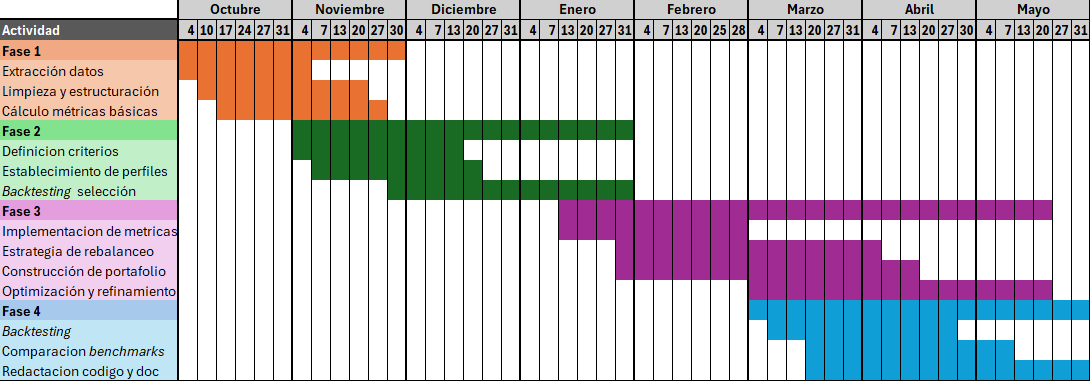
\includegraphics[width=0.92\textwidth]{figura_gantt.png}
\caption{Diagrama de Gantt del desarrollo del trabajo}
\label{fig:gantt}
\end{figure}
\fuente{Elaboración propia.}

El desarrollo se estructuró en cuatro fases secuenciales: adquisición y preparación de datos, selección multicriterio, optimización y rebalanceo, y validación empírica con análisis de resultados. Como complemento a estas fases se incorporaron actividades de trazabilidad, generación de figuras, documentación de limitaciones y reportes de cumplimiento de objetivos, ya que estas evidencias permiten presentar el trabajo de manera más verificable frente a evaluadores.

\clearpage
\section{Alcance y Limitaciones}

El trabajo de grado se limita a un universo específico de activos financieros, siendo estos ETFs listados y negociados en el mercado estadounidense. El modelo contempla posiciones largas, rebalanceo periódico y estrategias de portafolio adecuadas para un inversionista con horizonte de mediano o largo plazo. No se consideran ventas en corto, opciones, apalancamiento operativo, impuestos, ejecución real de órdenes ni asesoría financiera personalizada.

La principal limitación del trabajo corresponde a la disponibilidad y calidad de los datos. Los experimentos finales utilizan un universo público aproximado \textit{point-in-time}; esta aproximación mejora la trazabilidad frente a un universo completamente estático, pero no equivale a una base institucional libre de sesgo de supervivencia. Durante el desarrollo también se intentó contactar a CRSP (\textit{Center for Research in Security Prices}) \textit{Research Data Products} para consultar la posibilidad de una licencia académica; sin embargo, no fue posible concretar el acceso porque la negociación debía realizarse directamente desde la institución educativa. Esta situación dejó por fuera una fuente institucional que habría permitido mejorar la reconstrucción histórica del universo invertible. Adicionalmente, aunque el objetivo general contempla \textit{tracking error} y \textit{expense ratio}, las ejecuciones empíricas no contaron con cobertura completa para estos criterios, por lo cual el cumplimiento del objetivo general se considera parcial.

Una lectura relevante de la selección es el tamaño final del conjunto obtenido. Con los objetivos revisados, la cardinalidad deja de ser una meta fija y pasa a interpretarse como evidencia del grado de reducción logrado. En la prueba principal se obtuvo un promedio de 4.43 activos seleccionados por rebalanceo, mientras que en la validación ampliada el promedio fue de 5.29. Esta evidencia respalda que el sistema reduce el universo a un conjunto manejable para pequeños inversionistas, aunque también sugiere revisar en trabajos futuros si se desea mayor diversificación.



El alcance también se delimita desde el punto de vista del usuario esperado. El sistema está pensado como una herramienta académica y de apoyo exploratorio para inversionistas o analistas con interés en construir portafolios diversificados de ETFs, no como una plataforma de asesoría financiera personalizada. Por esta razón, los resultados no deben interpretarse como recomendación de compra o venta, sino como evidencia de comportamiento histórico bajo reglas específicas de selección y rebalanceo.

La interpretación de los resultados debe considerar que el mercado estadounidense durante 2021--2025 tuvo condiciones particulares, incluyendo recuperación postpandemia, cambios en tasas de interés, episodios de volatilidad y una fuerte concentración de retornos en algunos segmentos del mercado. Estos elementos afectan la comparación frente a SPY y al portafolio 60/40. Por ello, el hecho de que la estrategia multicriterio no supere a dichos \textit{benchmarks} no implica que el enfoque carezca de valor metodológico; indica que, bajo la configuración evaluada, la clasificación y asignación implementadas no generaron una ventaja robusta frente a alternativas simples.

\clearpage
\section{Implementación del Sistema de Clasificación Multicriterio}

El desarrollo del sistema de clasificación multicriterio mediante ELECTRE Tri constituye el centro metodológico del primer objetivo específico de esta investigación. La implementación se fundamenta en la adaptación de la metodología propuesta por Xidonas et al. (Xidonas, Mavrotas y Psarras, 2009) al mercado específico de ETFs, considerando las particularidades estructurales y operativas de estos instrumentos financieros que los diferencian de las acciones individuales tradicionalmente analizadas en la literatura MCDM.

La arquitectura del sistema se organizó como un flujo de trabajo en Python compuesto por módulos de datos, cálculo de características, clasificación, optimización, validación y reporte. Entre los componentes más relevantes se encuentran el cálculo de métricas financieras, la integración del \textit{pipeline} de selección, la validación de cumplimiento de objetivos, el corredor experimental y la generación automática de figuras. Esta estructura permite separar la clasificación ELECTRE de la asignación de pesos, evitando confundir el método multicriterio con un optimizador de portafolios.

La implementación se desarrolló de manera incremental. Primero se construyeron funciones para cargar datos y calcular métricas financieras. Después se integró la clasificación ELECTRE Tri con perfiles y criterios de decisión. Posteriormente se conectó la selección con estrategias de portafolio y rebalanceo. Finalmente se agregaron reportes, figuras y validaciones de cumplimiento de objetivos. Esta evolución refleja un desarrollo gradual propio de un proyecto aplicado: cada fase dependía de que la anterior produjera salidas consistentes.

Un aspecto importante de la implementación fue la trazabilidad. Cada experimento genera archivos con métricas de desempeño, curvas de capital, caídas, activos seleccionados por rebalanceo y resúmenes de cumplimiento. Esto permite reconstruir la cadena de decisiones desde los datos iniciales hasta las conclusiones. En un trabajo de grado aplicado, esta trazabilidad es tan importante como el resultado financiero, porque permite que un evaluador revise si las conclusiones están respaldadas por evidencia verificable.

Como complemento del documento escrito, el repositorio del proyecto en \textit{GitHub} se incorpora como entregable digital. Allí queda organizado el código fuente, los scripts de ejecución, las pruebas automatizadas, la documentación técnica y los archivos generados para la validación. Este entregable facilita la revisión del trabajo y permite que la metodología pueda ser replicada o ajustada posteriormente.


\begin{figure}[H]
\centering
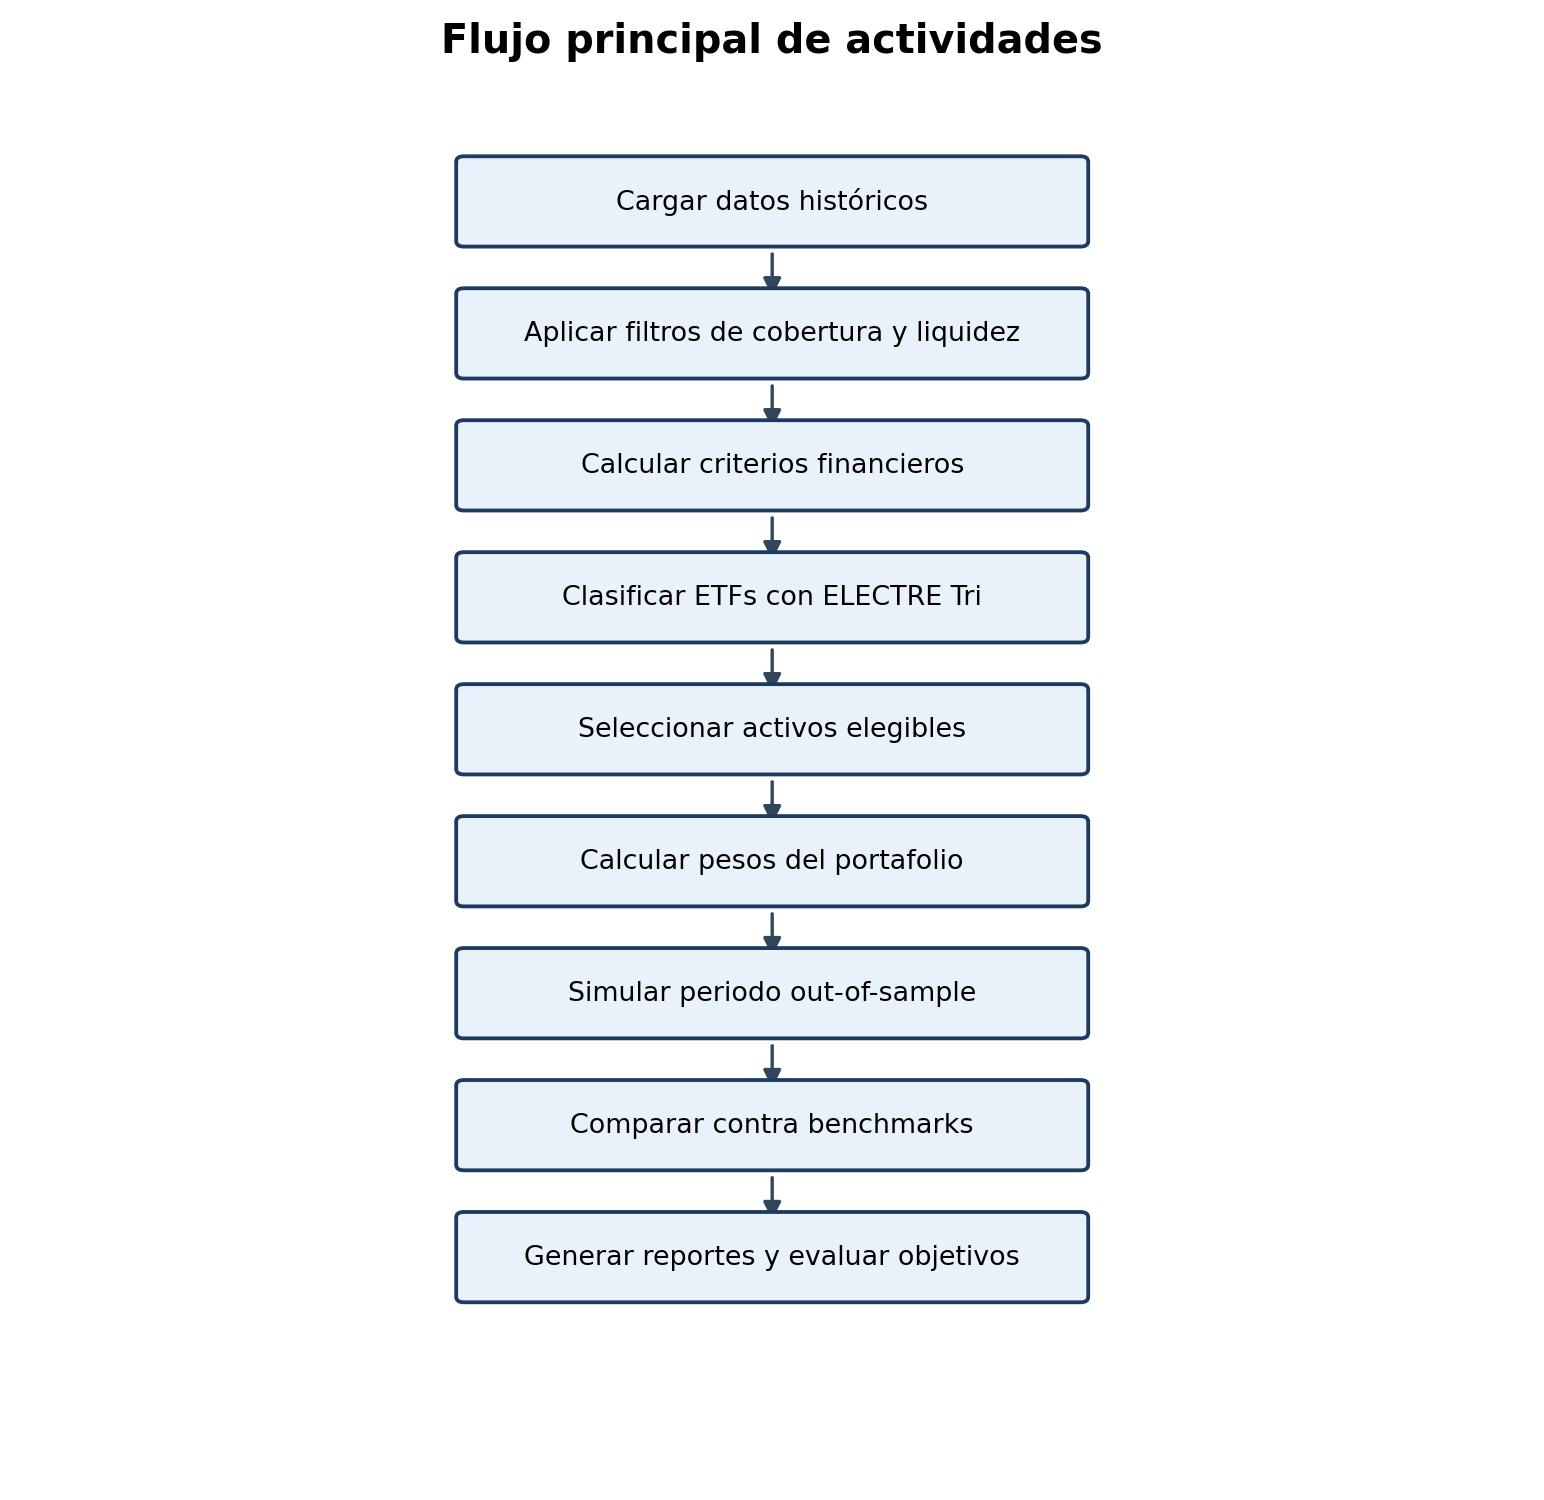
\includegraphics[width=0.92\textwidth]{flujo_trabajo_sistema.png}
\caption{Flujo de trabajo del sistema implementado}
\label{fig:componentes}
\end{figure}
\fuente{Elaboración propia a partir de la implementación en Python.}

\subsection{Definición de Categorías y Umbrales de Clasificación}

Se siguen los lineamientos de la metodología ELECTRE Tri, donde se determinan a priori categorías de clasificación. En este caso se establecieron tres categorías ordenadas que reflejan la calidad relativa de los ETFs en el universo de análisis: excelentes, aceptables y rechazados. Estas categorías permiten que el resultado del modelo sea interpretable y conectable con la etapa posterior de construcción del portafolio.

\begin{table}[H]
\centering
\caption{Categorías usadas para interpretar la clasificación ELECTRE}
\label{tab:categorias_electre}
\begin{tabular}{p{4cm}p{9cm}}
\toprule
\textbf{Categoría} & \textbf{Interpretación dentro del modelo} \\
\midrule
Excelentes & ETFs que superan los estándares multicriterio definidos y se consideran candidatos principales para el portafolio. \\
Aceptables & ETFs con desempeño razonable, pero no necesariamente superior en todos los criterios. \\
Rechazados & ETFs que no cumplen los estándares mínimos de calidad, liquidez, riesgo o eficiencia definidos para la selección. \\
\bottomrule
\end{tabular}
\end{table}
\fuente{Construido por el autor con base en ELECTRE Tri.}

\subsection{Resultados obtenidos durante la implementación}

La ejecución principal se realizó sobre el período 2021--2025, conservando la separación conceptual entre desarrollo 2021--2024 y validación 2025. La estrategia ELECTRE equiponderada obtuvo un CAGR agregado de 12.88\%, \textit{Sharpe Ratio} de 1.198 y máximo \textit{drawdown} de -7.54\%. Aunque este resultado es positivo en términos absolutos, queda por debajo de SPY y del portafolio 60/40 en desempeño ajustado por riesgo. Por esta razón, el resultado debe leerse como evidencia de funcionamiento y comparación reproducible del sistema, no como confirmación de superioridad del enfoque multicriterio.

La lectura de la prueba principal debe hacerse con cuidado. En términos absolutos, ELECTRE equiponderado alcanza una rentabilidad positiva y un \textit{drawdown} similar al de SPY, lo cual muestra que el sistema sí construye portafolios operativos. Sin embargo, el \textit{Sharpe Ratio} queda por debajo de SPY, del portafolio 60/40 y del universo equiponderado. Esta diferencia indica que la selección multicriterio, en su configuración actual, no logró transformar la reducción del universo en una mejora suficiente de rentabilidad ajustada por riesgo.

El tamaño de la selección deja una lectura importante para el trabajo. El modelo no entrega una cartera amplia en todas las fechas; más bien concentra el universo en pocos activos cuando las condiciones de los criterios son exigentes. Desde una mirada de Ingeniería Industrial, esto no se interpreta como un error aislado del algoritmo, sino como una señal del proceso: el filtro está siendo estricto y privilegia trazabilidad sobre amplitud. La contrapartida es clara. Si en una aplicación práctica se busca una diversificación mayor, habría que ajustar perfiles, umbrales o reglas finales sin perder el sentido de calidad que motivó la selección inicial.

\begin{table}[H]
\centering
\caption{Composición temporal del protocolo principal 2021--2025}
\label{tab:composicion_temporal_principal}
\begin{tabular}{p{3cm}p{1.5cm}p{8.5cm}}
\toprule
\textbf{Rebalanceo} & \textbf{n} & \textbf{ETFs elegidos} \\
\midrule
2024-02-29 & 4 & CDL, COM, COMT, COWZ \\
2024-05-31 & 1 & COMT \\
2024-08-31 & 2 & CGDV, CGUS \\
2024-11-30 & 2 & CGDV, CGUS \\
2025-02-28 & 5 & BUFR, CATH, CGDV, CGGR, CGUS \\
2025-05-31 & 7 & BUFR, CATH, CGDV, CGGO, CGGR, CGUS, CIBR \\
2025-08-31 & 10 & BUFD, BUFG, BUFR, CAPE, CATH, CGDV, CGGO, CGGR, CGUS, CIBR \\
\bottomrule
\end{tabular}
\end{table}
\fuente{Cálculo con \texttt{electre\_selection\_by\_rebalance.csv}, corrida principal.}

La tabla anterior muestra que la selección se mueve de forma gradual y no como una lista fija. En las primeras fechas el clasificador deja pasar muy pocos instrumentos, mientras que en 2025 aparece una apertura mayor del conjunto elegido. Para la lectura del primer objetivo, este detalle es importante: la reducción del universo sí ocurre, pero no mediante una cuota impuesta de activos. El resultado depende de la información disponible en cada rebalanceo y de la exigencia de los perfiles ELECTRE.


\begin{table}[H]
\centering
\caption{Resultados principales de la prueba 2021--2025}
\label{tab:resultados_principales}
\begin{tabular}{p{5.0cm}rrr}
\toprule
\textbf{Estrategia} & \textbf{CAGR} & \textbf{Sharpe} & \textbf{Caída máxima} \\
\midrule
ELECTRE equiponderado & 12.88\% & 1.198 & -7.54\% \\
ELECTRE mínima varianza & 12.47\% & 1.236 & -6.56\% \\
ELECTRE \textit{MaxSharpe} & 10.97\% & 1.034 & -7.62\% \\
SPY comprar y mantener & 23.32\% & 1.932 & -7.58\% \\
Portafolio 60/40 SPY-BND & 15.85\% & 1.964 & -3.80\% \\
Universo equiponderado & 11.98\% & 1.695 & -3.48\% \\
\bottomrule
\end{tabular}
\end{table}
\fuente{Elaboración propia con base en los resultados generados por el sistema.}

\begin{figure}[H]
\centering
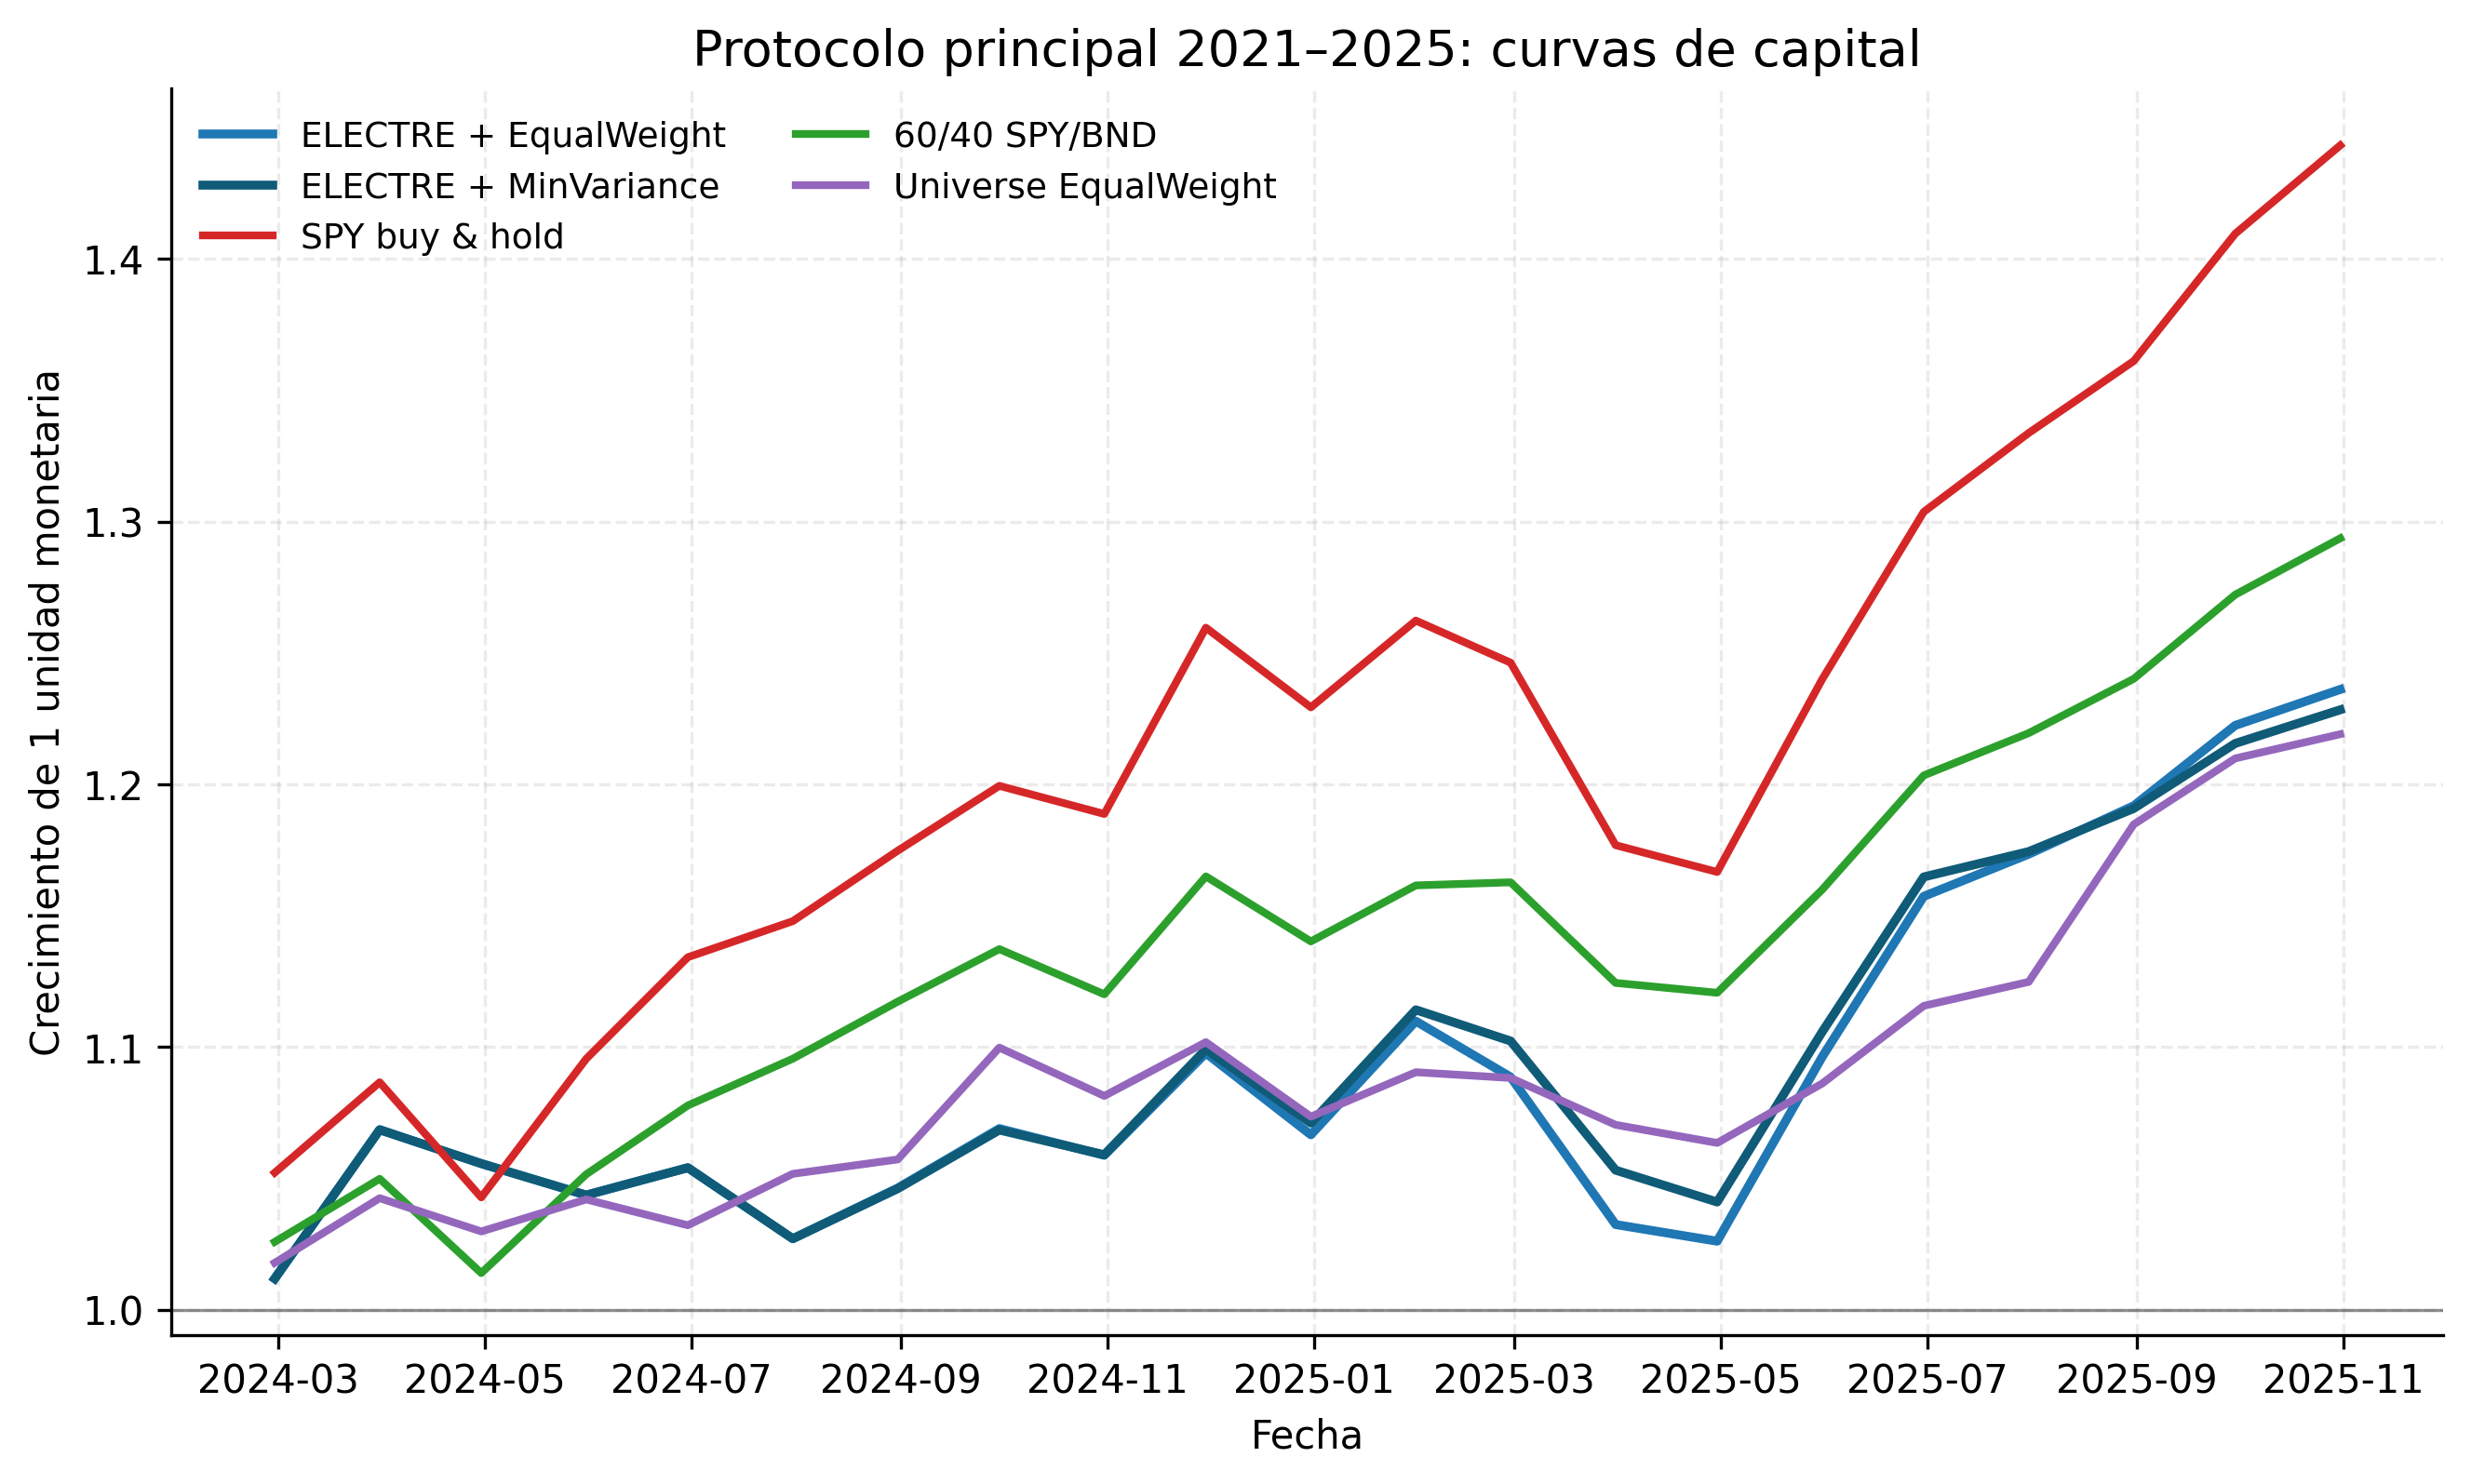
\includegraphics[width=0.92\textwidth]{evolucion_capital_principal.png}
\caption{Evolución del capital en la prueba principal}
\label{fig:capital_principal}
\end{figure}
\fuente{Elaboración propia.}

\begin{figure}[H]
\centering
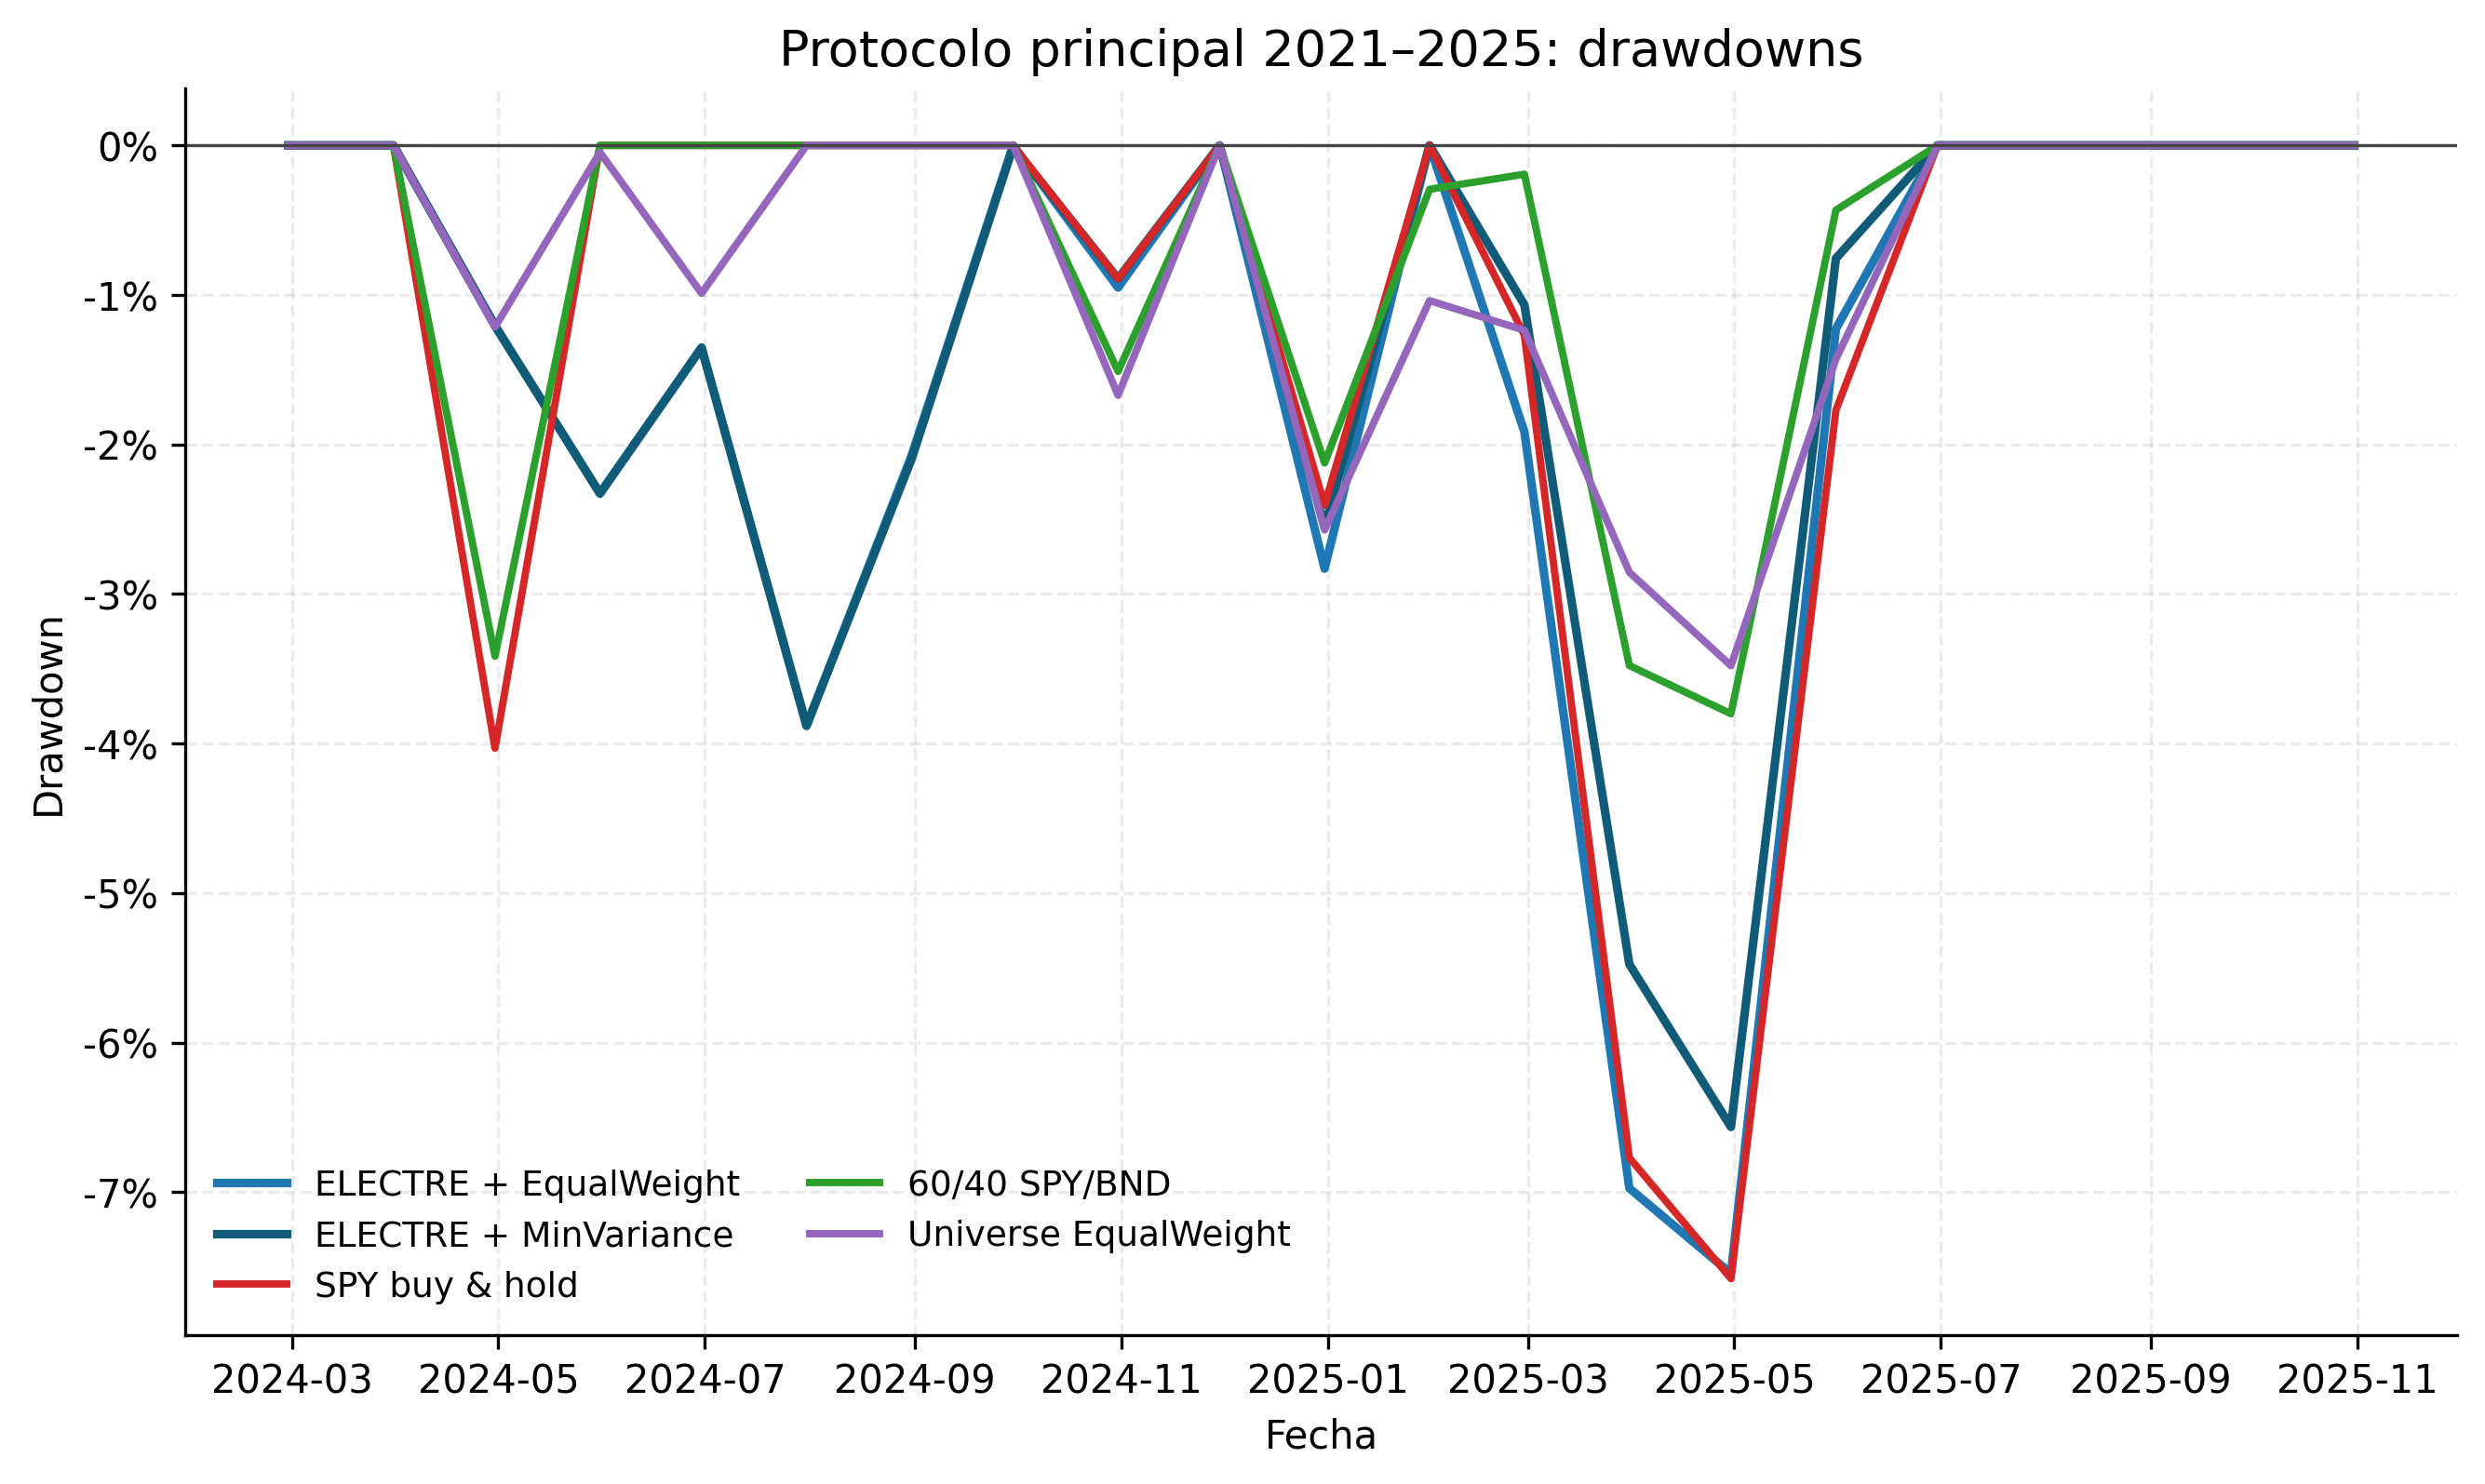
\includegraphics[width=0.92\textwidth]{caidas_prueba_principal.png}
\caption{Caídas acumuladas durante la prueba principal}
\label{fig:caidas_principal}
\end{figure}
\fuente{Elaboración propia.}

\begin{figure}[H]
\centering
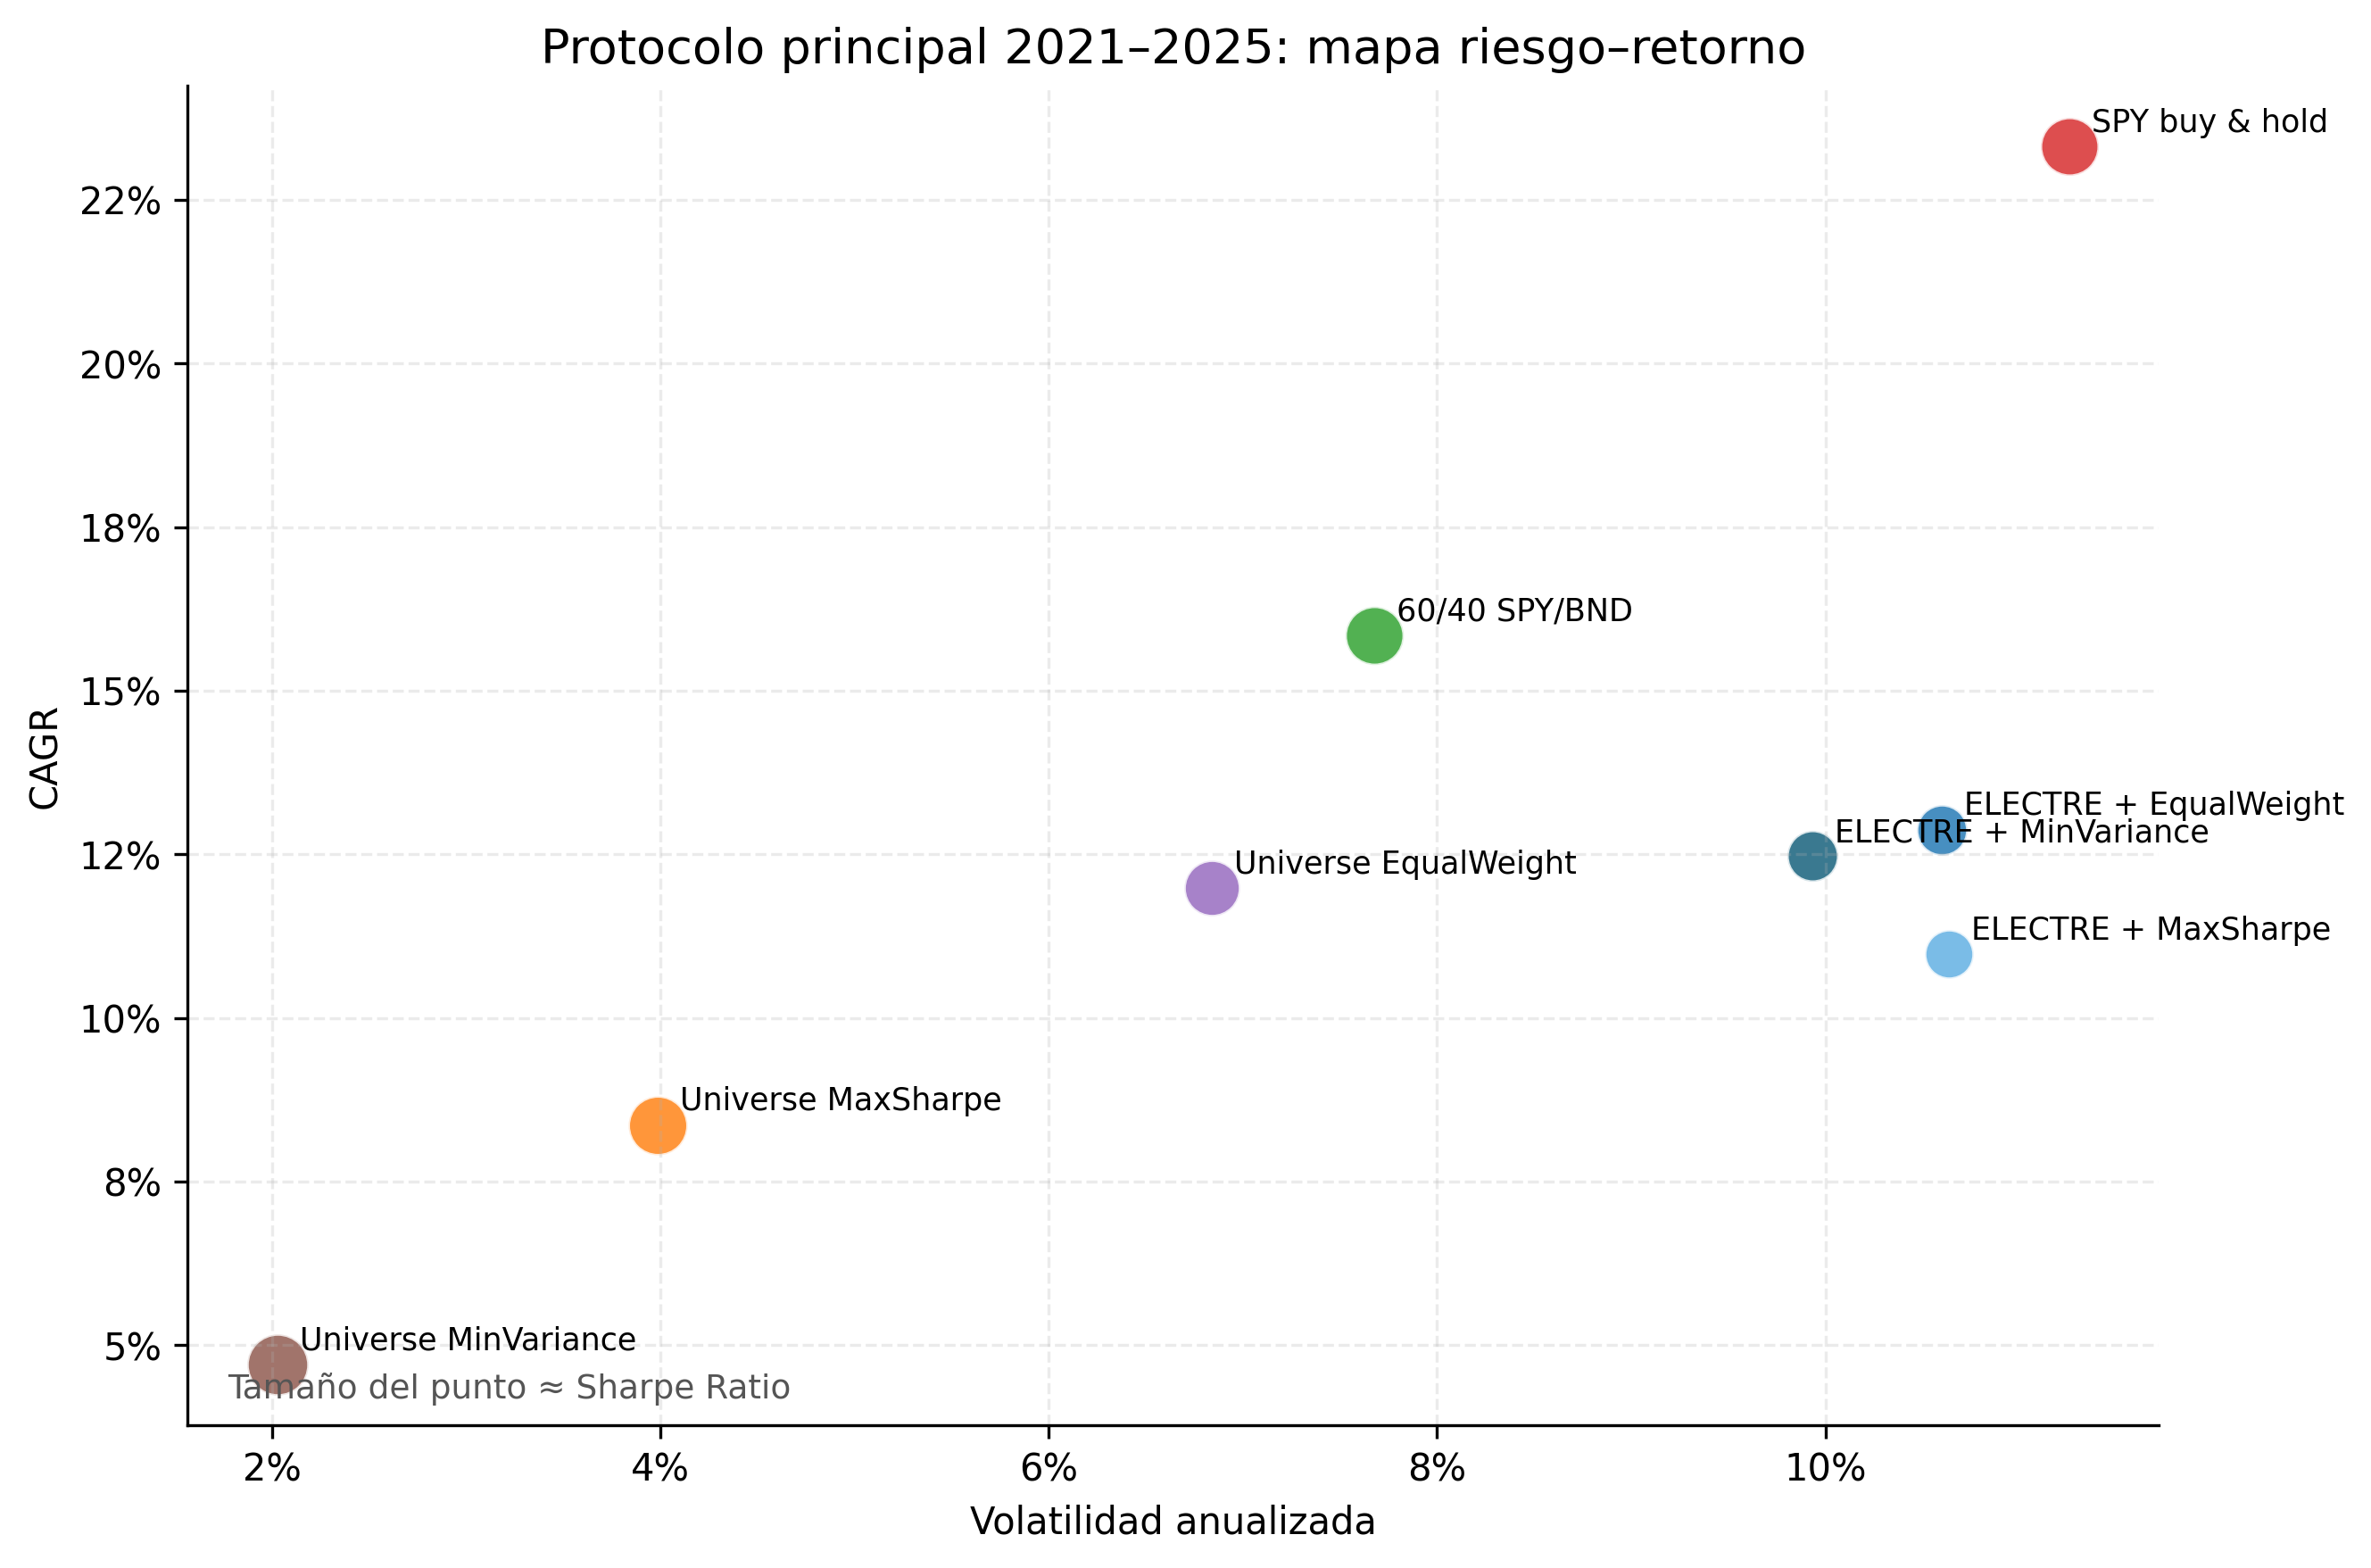
\includegraphics[width=0.92\textwidth]{riesgo_rentabilidad_principal.png}
\caption{Relación entre riesgo y rentabilidad en la prueba principal}
\label{fig:riesgo_rentabilidad}
\end{figure}
\fuente{Elaboración propia.}

\begin{figure}[H]
\centering
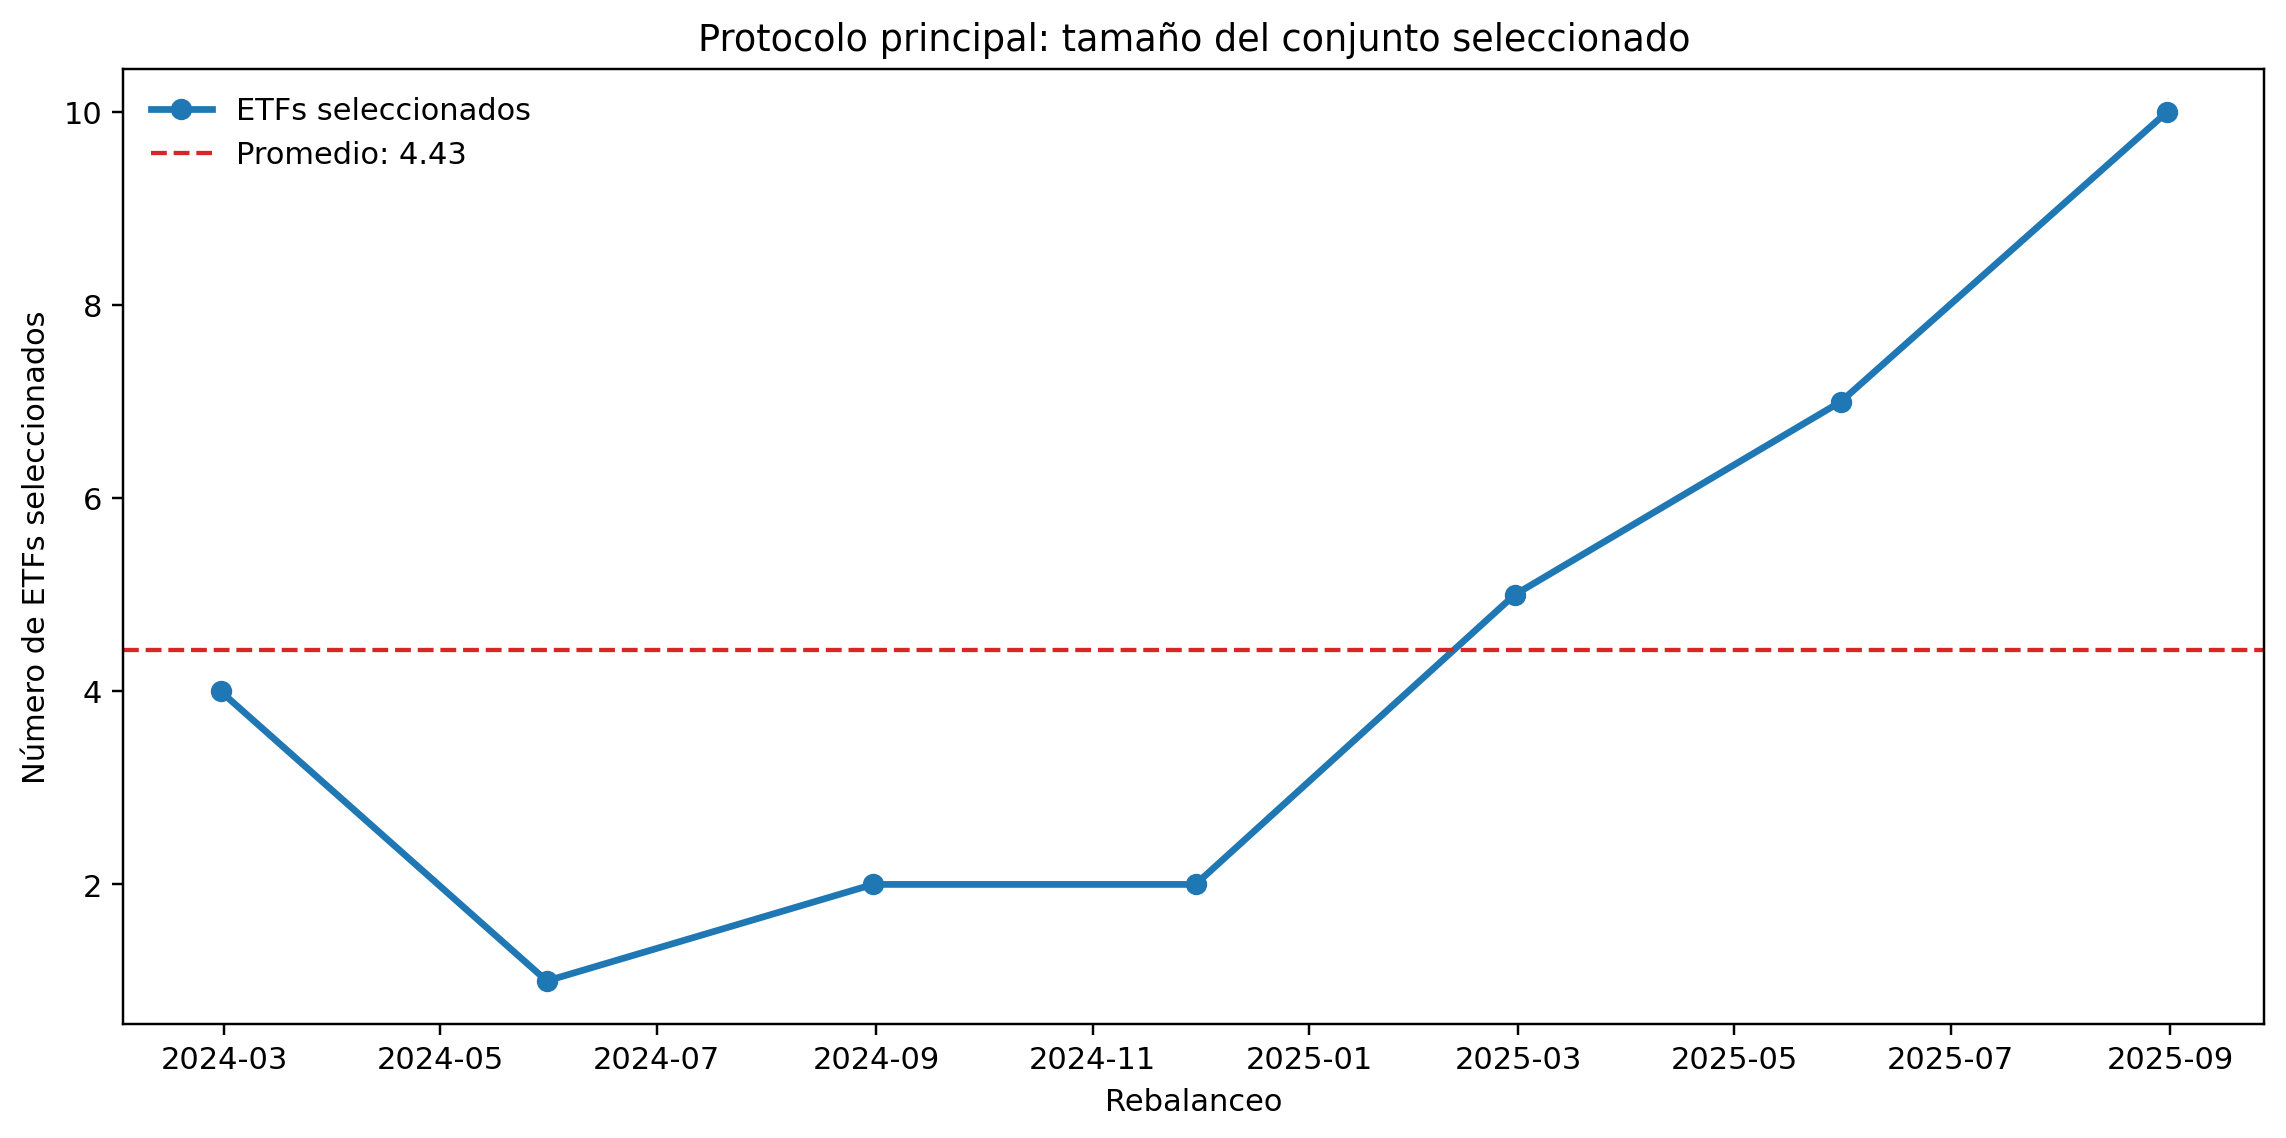
\includegraphics[width=0.92\textwidth]{numero_etfs_rebalanceo.png}
\caption{Número de ETFs seleccionados en cada rebalanceo}
\label{fig:cardinalidad}
\end{figure}
\fuente{Elaboración propia.}

\begin{table}[H]
\centering
\caption{Resumen de cardinalidad en la corrida principal 2021--2025}
\label{tab:cardinalidad_resumen_principal}
\begin{tabular}{p{5.2cm}p{2.8cm}}
\toprule
\textbf{Métrica} & \textbf{Valor} \\
\midrule
Rebalanceos con selección activa & 7 \\
Promedio de ETFs seleccionados & 4.43 \\
Mediana & 4 \\
Mínimo--Máximo & 1--10 \\
\bottomrule
\end{tabular}
\end{table}
\fuente{Recuento sobre \texttt{electre\_selection\_by\_rebalance.csv}, corrida principal.}

El resumen de cardinalidad confirma esa misma idea con números agregados. El promedio de 4.43 ETFs seleccionados es bajo frente a una cartera diversificada tradicional, pero es coherente con un filtro pensado para depurar un universo amplio antes de optimizar. En una implementación real, este punto sería una decisión de diseño: mantener una selección estricta o incorporar una regla adicional de tamaño mínimo.

\subsection{Validación ampliada y lectura de robustez}

La validación ampliada 2015--2025 se ejecutó para revisar la estabilidad del enfoque fuera del período principal. En esta prueba, ELECTRE equiponderado obtuvo un CAGR de 3.78\%, \textit{Sharpe Ratio} de 0.332 y caída máxima de -20.45\%, quedando por debajo de SPY, del portafolio 60/40 y del universo equiponderado. Esta lectura confirma que la metodología construida es útil para evaluar y documentar decisiones, pero que su configuración actual no demuestra una ventaja robusta frente a estrategias simples.

La validación ampliada obliga a mirar el modelo con más calma. Al extender el período a 2015--2025, el desempeño de las estrategias ELECTRE se debilita frente a SPY, 60/40 y el universo equiponderado. Esta evidencia no anula la metodología, pero sí evita una conclusión apresurada basada solo en una ventana corta. En términos de proyecto de grado, el resultado es útil precisamente porque muestra dónde funciona el sistema, dónde pierde fuerza y qué ajustes tendría sentido estudiar después.

Para esta validación ampliada se ejecutaron 31 rebalanceos, con tamaño medio del conjunto seleccionado de 5.29 activos, mínimo 1 y máximo 11. El resultado no se interpreta como inestabilidad técnica del \textit{pipeline}, sino como evidencia de que la selección mantiene núcleos de referencia y varía por régimen.

\begin{table}[H]
\centering
\caption{\textit{Tickers} más recurrentes en la validación ampliada 2015--2025}
\label{tab:recurrentes_ampliada}
\begin{tabular}{p{1.8cm}p{2.2cm}p{3.2cm}p{4.8cm}}
\toprule
\textbf{\textit{Ticker}} & \textbf{Apariciones} & \textbf{Porcentaje de rebalanceos} & \textbf{Lectura} \\
\midrule
CDC & 19 & 61.3\% & Presencia constante en periodos con mayor persistencia de criterio financiero. \\
CIBR & 17 & 54.8\% & Núcleo central de selección en fases de continuidad estratégica. \\
CFO & 17 & 54.8\% & Persistencia alta ligada a liquidez y estabilidad de desempeño. \\
CFA & 14 & 45.2\% & Aporte recurrente en fases de rotación del bloque tecnológico-financiero. \\
CGW & 13 & 41.9\% & Componente estable en etapas de selección de calidad por segmento. \\
\bottomrule
\end{tabular}
\end{table}
\fuente{Conteos de apariciones sobre los 31 rebalanceos de la corrida de robustez.}

La recurrencia de estos \textit{tickers} no debe leerse como una recomendación de compra. Su aporte dentro del documento es más metodológico: permite ver que el sistema no selecciona activos completamente distintos en cada fecha, sino que conserva algunos núcleos cuando los criterios vuelven a favorecerlos. Esa estabilidad parcial ayuda a entender mejor el comportamiento del clasificador en una ventana larga.

\subsection{Lectura integrada de los resultados}

Al mirar en conjunto la prueba principal, la validación ampliada y las tablas de selección, la conclusión queda más matizada que una simple comparación de rentabilidades. El sistema sí cumple una función clara: ordena un universo grande de ETFs, aplica criterios homogéneos por fecha de rebalanceo y deja una ruta replicable para pasar de datos históricos a portafolios evaluables. Esa parte del trabajo es valiosa porque convierte una decisión normalmente dispersa en un proceso documentado.

También hay límites que no conviene suavizar. La selección quedó concentrada en varias fechas y el desempeño ajustado por riesgo no superó a referentes simples como SPY o el portafolio 60/40. Desde una lectura de Ingeniería Industrial, este resultado muestra que el diseño del sistema y su resultado financiero no son la misma cosa. El proceso puede estar bien construido y, aun así, necesitar mejores datos, criterios más completos o reglas de asignación más robustas.

Por eso el aporte principal del trabajo se ubica en la trazabilidad del método. La tesis no plantea que ELECTRE vence siempre a las estrategias tradicionales. Lo que muestra es más concreto: se puede construir un flujo reproducible para seleccionar ETFs, revisar su comportamiento, compararlos contra \textit{benchmarks} y detectar qué parte del sistema requiere ajuste. Esta lectura es más prudente y queda mejor conectada con los resultados obtenidos.

Las figuras siguientes complementan esta lectura porque muestran el comportamiento de las estrategias y la relación entre las categorías ELECTRE y el desempeño posterior. Su función no es decorar el resultado, sino permitir una revisión visual de lo que las tablas resumen: desempeño, estabilidad y límites del clasificador bajo las ventanas evaluadas.


\begin{figure}[H]
\centering
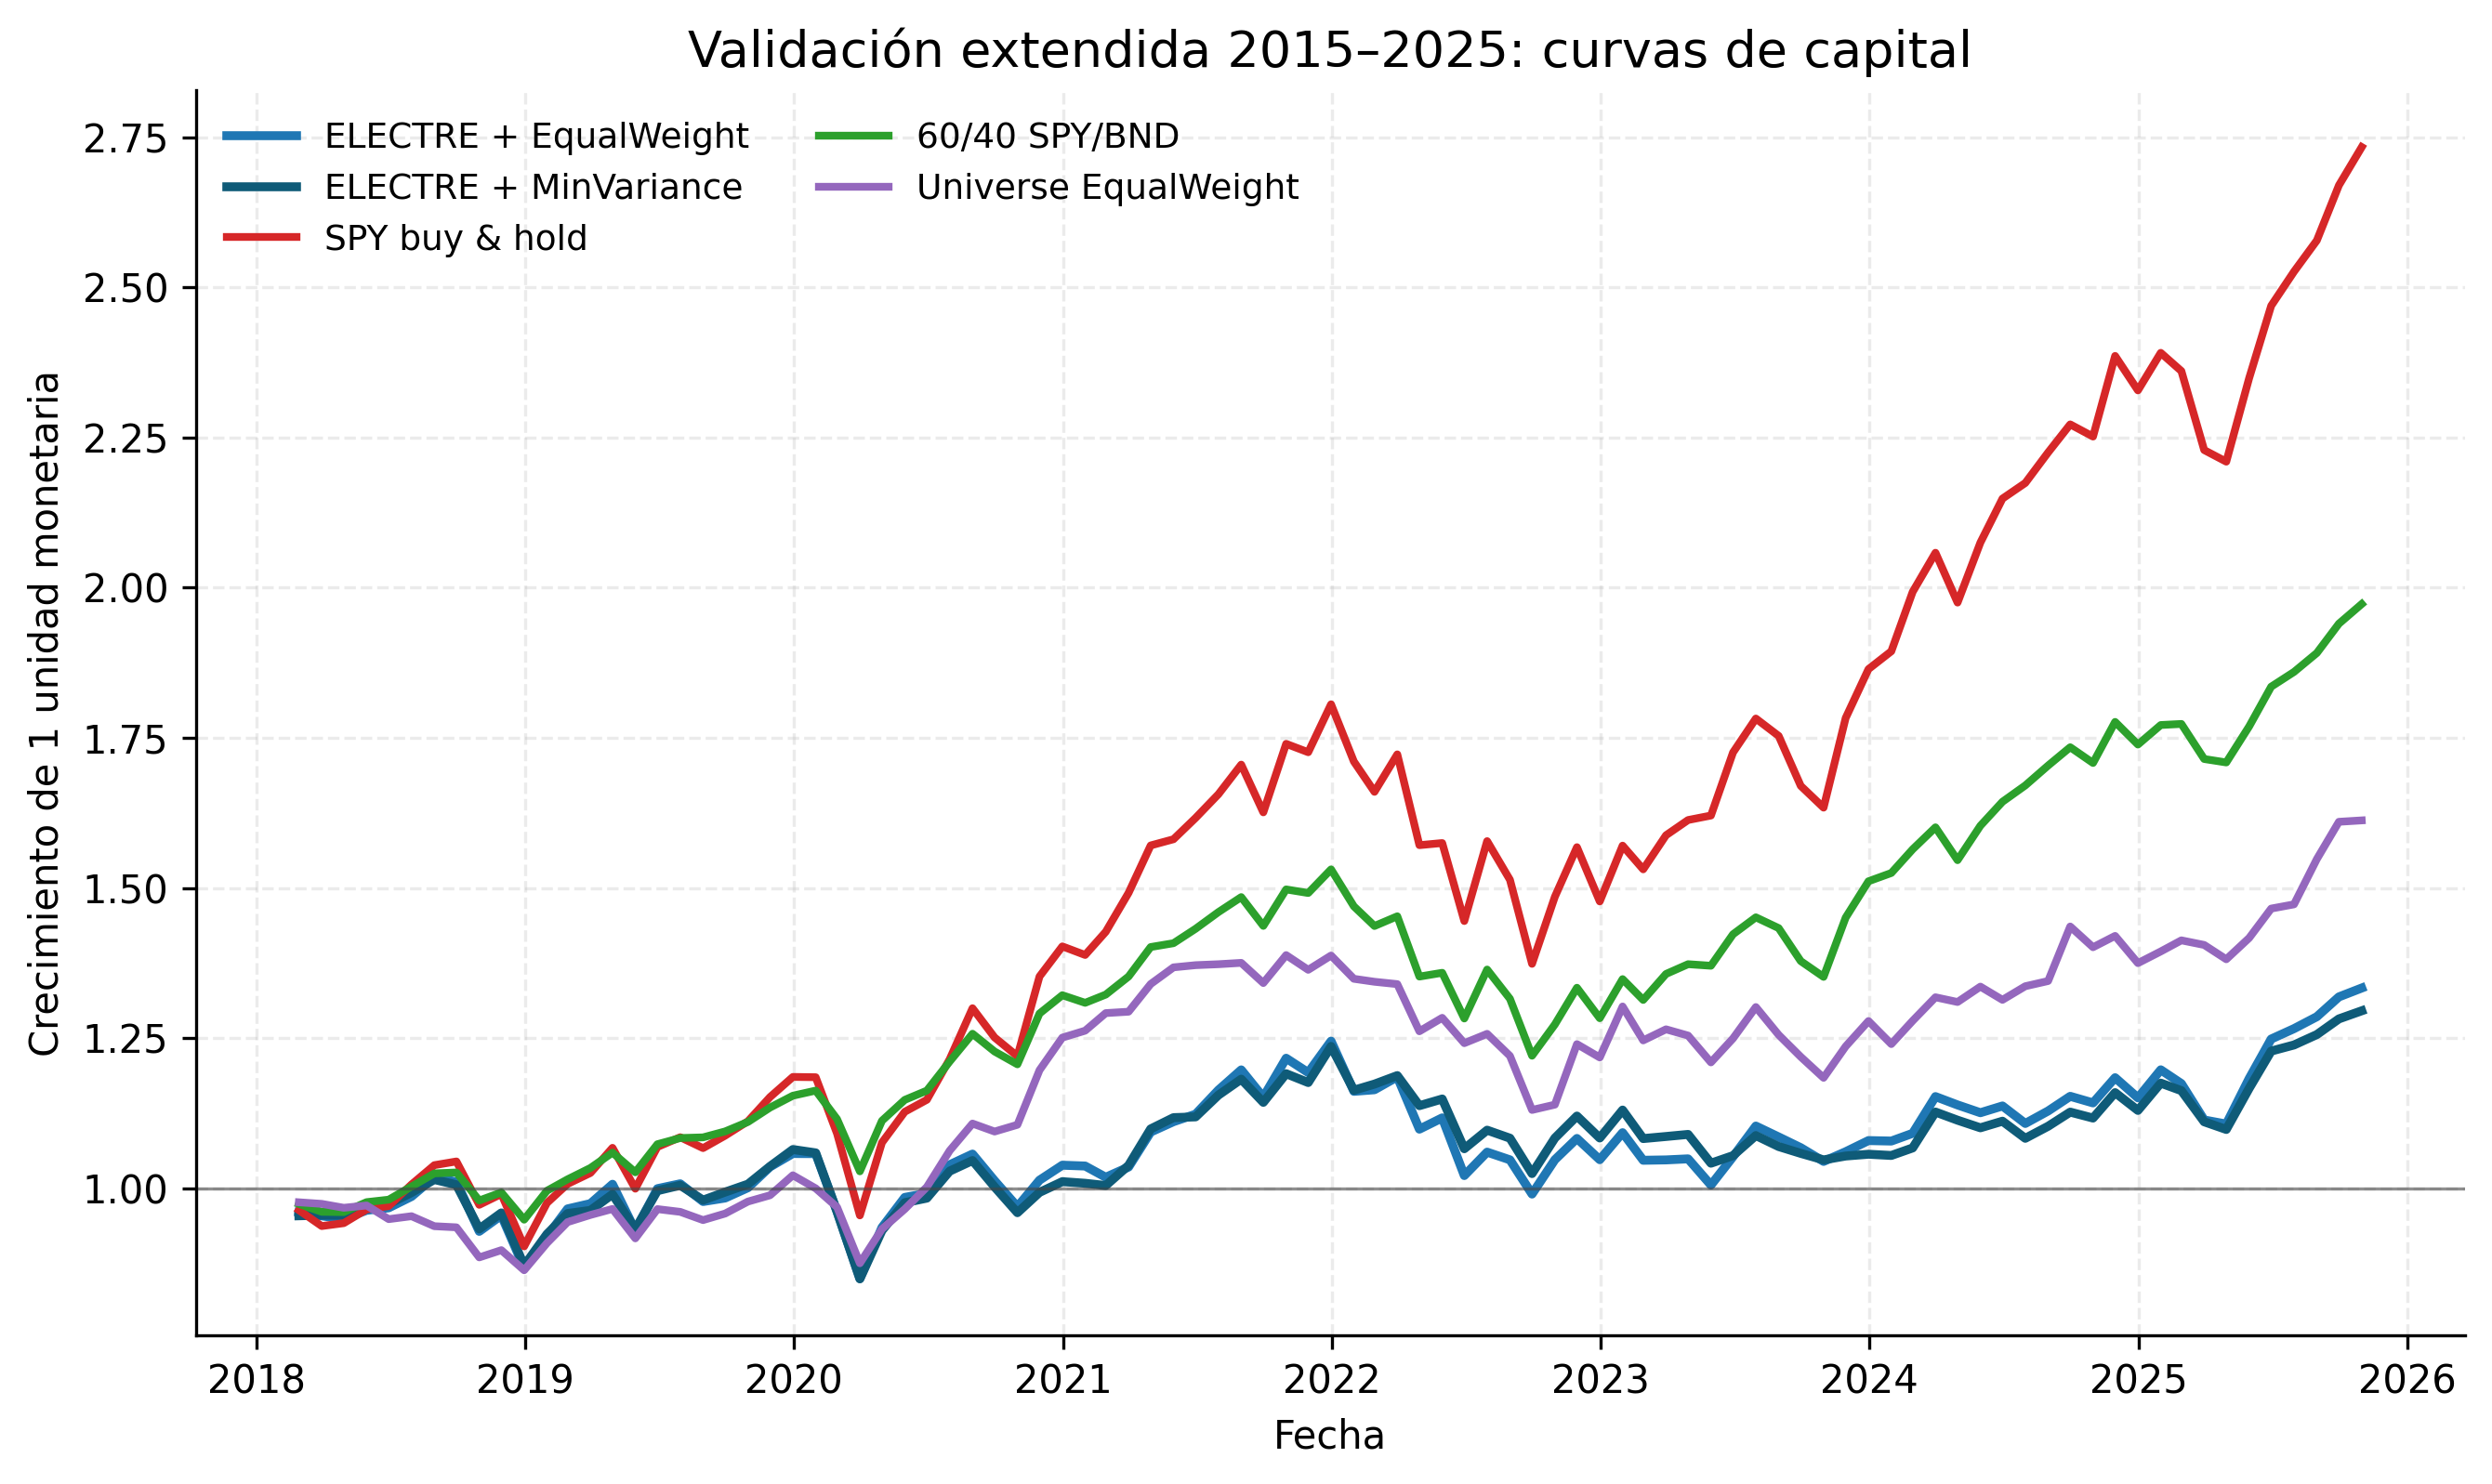
\includegraphics[width=0.92\textwidth]{evolucion_capital_ampliada.png}
\caption{Comportamiento de las estrategias en la validación ampliada}
\label{fig:capital_ampliada}
\end{figure}
\fuente{Elaboración propia.}

\begin{figure}[H]
\centering
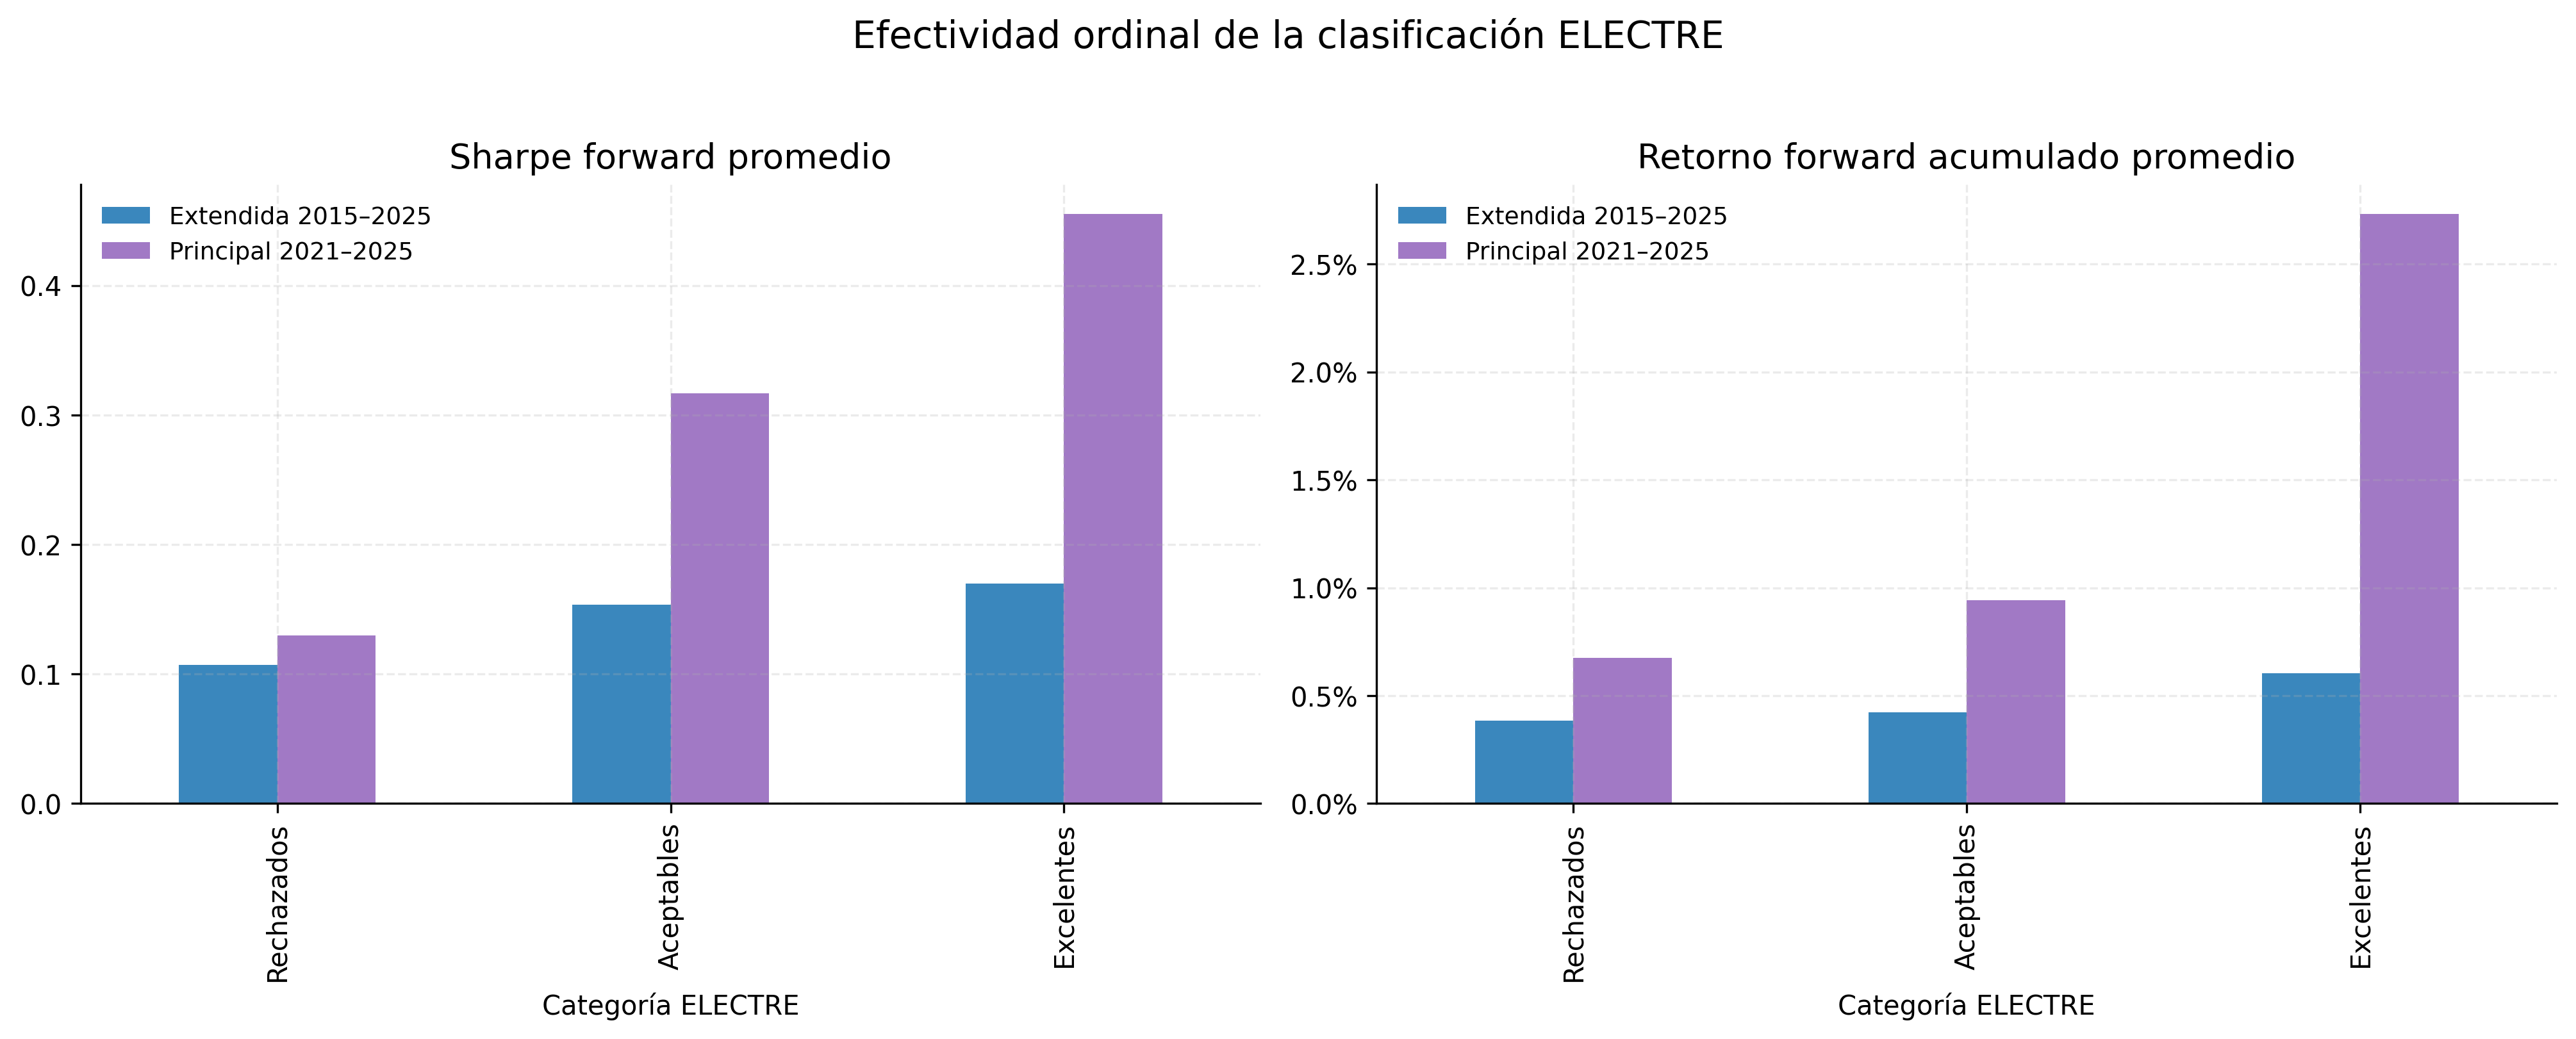
\includegraphics[width=0.92\textwidth]{lectura_categorias_electre.png}
\caption{Lectura de las categorías ELECTRE frente al desempeño posterior}
\label{fig:categorias}
\end{figure}
\fuente{Elaboración propia.}

\begin{figure}[H]
\centering
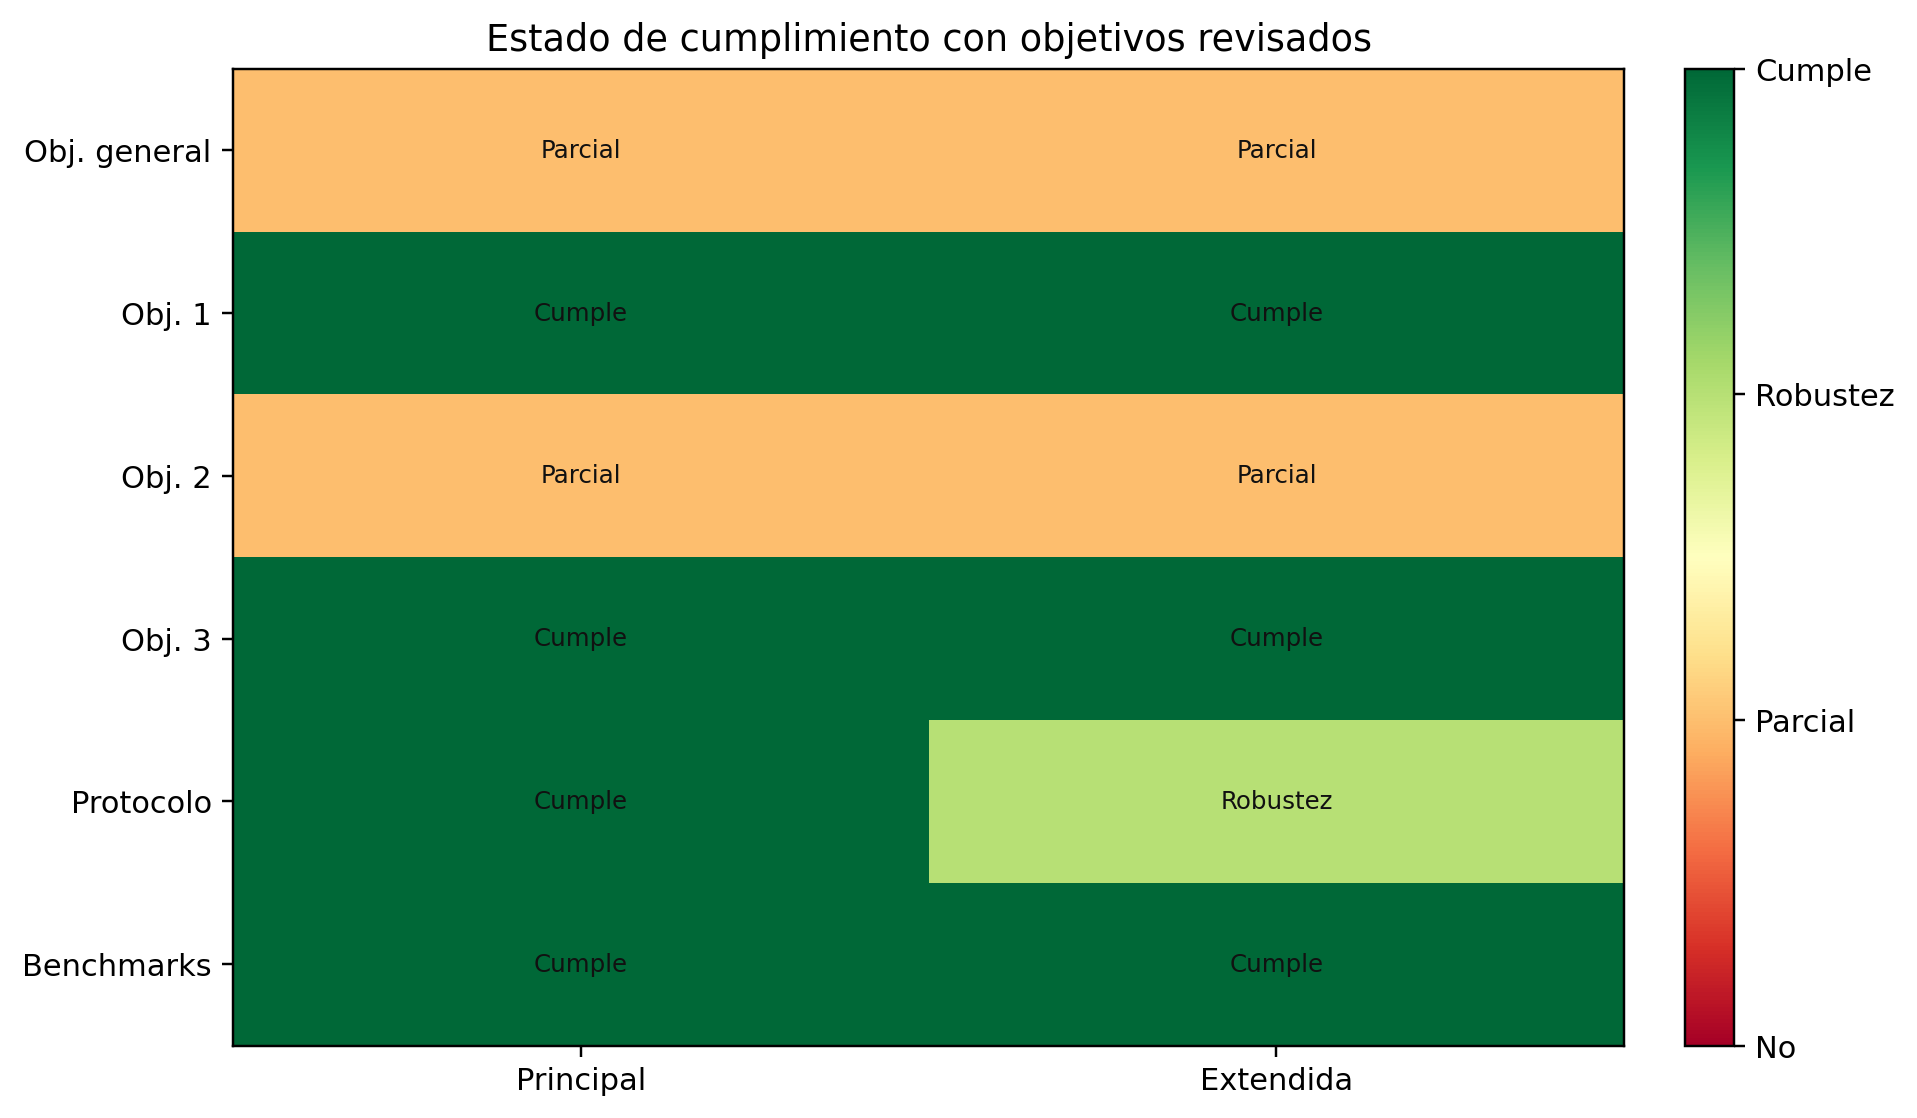
\includegraphics[width=0.92\textwidth]{cumplimiento_objetivos.png}
\caption{Estado de cumplimiento de los objetivos del trabajo}
\label{fig:cumplimiento}
\end{figure}
\fuente{Elaboración propia.}

\subsection{Cierre de implementación y trabajo futuro}

El proyecto permitió desarrollar un sistema funcional de clasificación, optimización y validación de portafolios de ETFs. Como parte de la validación técnica, el sistema fue evaluado mediante pruebas automatizadas y los resultados principales quedaron documentados en métricas, curvas de capital, caídas, selección por rebalanceo y cumplimiento de objetivos. En conjunto, la evidencia permite sostener que la contribución principal del trabajo es metodológica y diagnóstica: se valida un proceso reproducible para reducir el universo de ETFs, construir portafolios y comparar su desempeño frente a \textit{benchmarks} tradicionales.

Como trabajo futuro se recomienda completar la integración de \textit{tracking error} y \textit{expense ratio} con fuentes confiables, estudiar reglas opcionales de diversificación y tamaño mínimo cuando el usuario las requiera, fortalecer los grupos comparables dentro de ELECTRE Tri, mejorar el manejo de restricciones de exposición y construir una arquitectura de datos regulatoria enriquecida con fuentes institucionales como CRSP \textit{Research Data Products}, SEC (\textit{Securities and Exchange Commission}) N-PORT (\textit{Monthly Portfolio Investments Report}), N-CEN (\textit{Annual Report for Registered Investment Companies}), EDGAR (\textit{Electronic Data Gathering, Analysis, and Retrieval}) y OpenFIGI (\textit{Open Financial Instrument Global Identifier}). En particular, el acceso a CRSP debería gestionarse desde la universidad o mediante un convenio académico, porque durante el desarrollo individual del proyecto no fue posible obtener la licencia directamente. Estas mejoras permitirían ampliar el alcance del sistema sin alterar la contribución metodológica demostrada.

En relación con el objetivo general, el trabajo logra desarrollar una herramienta integrada de selección y optimización basada en ETFs, aunque su validación queda parcialmente limitada por la ausencia completa de \textit{tracking error} y \textit{expense ratio} en las ejecuciones empíricas. En relación con el primer objetivo específico, se implementa el sistema de clasificación multicriterio y se reduce el universo a un conjunto manejable. En relación con el segundo objetivo, se desarrolla el análisis histórico de los ETFs elegibles y se obtiene evidencia parcial de consistencia ordinal. Finalmente, respecto al tercer objetivo, se realiza el \textit{benchmarking} frente a estrategias tradicionales sin presentar la comparación como promesa de superioridad.

Estas conclusiones responden directamente a los objetivos planteados y evidencian que el trabajo no se limita a proponer un modelo teórico o idealizado. El aporte principal está en el diseño, implementación y evaluación de un sistema aplicado, cuyos resultados permiten reconocer tanto sus aciertos como sus limitaciones. Teniendo esto en cuenta, fue posible identificar en qué condiciones la metodología ofrece un mejor desempeño y cuáles son las brechas que deberían abordarse en futuras versiones. En ese sentido, el proyecto refleja el valor práctico de la Ingeniería Industrial: analizar un problema complejo, estructurar una solución verificable y utilizar la evidencia obtenida para fortalecer la toma de decisiones.


\clearpage
\section{Bibliografía}
\label{sec:bibliografia}

\apa{Albadvi, A., Chaharsooghi, S. K., \& Esfahanipour, A. (2006). Decision making in stock trading: An application of PROMETHEE. \textit{European Journal of Operational Research, 177}(2), 673--683. https://doi.org/10.1016/j.ejor.2005.11.022}

\apa{Ballestero, E., Bravo, M., Pérez-Gladish, B., Arenas-Parra, M., \& Plà-Santamaria, D. (2012). Socially responsible investment: A multicriteria approach to portfolio selection combining ethical and financial objectives. \textit{European Journal of Operational Research, 216}(2), 487--494. https://doi.org/10.1016/j.ejor.2011.07.011}

\apa{Black, F., \& Litterman, R. (1992). Global portfolio optimization. \textit{Financial Analysts Journal}.}

\apa{Brans, J. P., \& Mareschal, B. (2005). PROMETHEE methods. En J. Figueira, S. Greco, \& M. Ehrgott (Eds.), \textit{Multiple criteria decision analysis: State of the art surveys}.}

\apa{Brans, J. P., \& Vincke, P. (1985). A preference ranking organisation method. \textit{Management Science, 31}(6), 647--656. https://doi.org/10.1287/mnsc.31.6.647}

\apa{Cohen, S., \& Del Valle, J. (2025). \textit{Decoding active ETFs: How the growth of active ETFs is unlocking innovation and opportunity for investors}. BlackRock.}

\apa{DeMiguel, V., Garlappi, L., \& Uppal, R. (2009). Optimal versus naive diversification: How inefficient is the 1/N portfolio strategy? \textit{The Review of Financial Studies}.}

\apa{Elton, E. J., Gruber, M. J., Brown, S. J., \& Goetzmann, W. N. (2014). \textit{Modern portfolio theory and investment analysis} (9th ed.).}

\apa{Emamat, M. S. M. M., Mikhailov, L., \& Alijamaat, A. (2022). Using ELECTRE Tri and FlowSort methods in stock portfolio selection.}

\apa{Hwang, C.-L., \& Yoon, K. (1981). Methods for multiple attribute decision making. En \textit{Multiple attribute decision making} (pp. 58--191). Springer. https://doi.org/10.1007/978-3-642-48318-9\_3}

\apa{Investment Company Institute. (2025). \textit{Investment Company Fact Book: A review of trends and activities in the investment company industry}.}

\apa{Kritzman, M., Page, S., \& Turkington, D. (2010). In defense of optimization: The fallacy of 1/N. \textit{Financial Analysts Journal}.}

\apa{Ledoit, O., \& Wolf, M. (2004). A well-conditioned estimator for large-dimensional covariance matrices. \textit{Journal of Multivariate Analysis, 88}(2), 365--411.}

\apa{López de Prado, M. (2016). Building diversified portfolios that outperform out of sample.}

\apa{Markowitz, H. (1952). Portfolio selection. \textit{The Journal of Finance}.}

\apa{Markowitz, H. (1959). \textit{Portfolio selection: Efficient diversification of investments}.}

\apa{Michaud, R. O. (1998). \textit{Efficient asset management}.}

\apa{Pendaraki, K., Zopounidis, C., \& Doumpos, M. (2005). On the construction of mutual fund portfolios: A multicriteria methodology and an application to the Greek market of equity mutual funds. \textit{European Journal of Operational Research, 163}(2), 462--481. https://doi.org/10.1016/j.ejor.2003.10.022}

\apa{Roy, B. (1968). Classement et choix en présence de points de vue multiples: La méthode ELECTRE. \textit{Revue française d'informatique et de recherche opérationnelle, 2}(8), 57--75. https://doi.org/10.1051/ro/196802V100571}

\apa{Roy, B. (1993). Decision science or decision-aid science? \textit{European Journal of Operational Research}.}

\apa{Roy, B., \& Bouyssou, D. (1993). \textit{Aide multicritère à la décision: Méthodes et cas}.}

\apa{Saaty, T. L. (1980). \textit{The analytic hierarchy process}.}

\apa{Sharpe, W. F. (1964). Capital asset prices: A theory of market equilibrium under conditions of risk. \textit{The Journal of Finance}.}

\apa{Spronk, J., Steuer, R. E., \& Zopounidis, C. (2005). Multicriteria decision aid/analysis in finance.}

\apa{Steuer, R. E., \& Na, P. (2003). Multiple criteria decision making combined with finance: A categorized bibliographic study.}

\apa{Tiryaki, F., \& Ahlatcioglu, B. (2009). Fuzzy portfolio selection using fuzzy analytic hierarchy process.}

\apa{Tsalikis, E., \& Papadopoulos, S. (2019). ETFs: Performance, tracking errors and their determinants in Europe and the USA.}

\apa{Vuorela, T. (2024). Assessing the impact of AI-managed ETFs on investment performance and risk compared to benchmark index.}

\apa{Xidonas, P., Mavrotas, G., \& Psarras, J. (2009). A multicriteria methodology for equity selection using financial analysis.}

\apa{Zopounidis, C., \& Doumpos, M. (2013). Multicriteria decision systems for financial problems.}
\end{document}
